\documentclass[asp1.tex]{subfiles}
\begin{document}

\section{BWL}
\subsection{Unternehmensphilosophie}
Grundelemente einer Unternehmensphilosophie sind die
\begin{itemize}
    \item Grundwerte und Überzeugungen
    \item Standards und Symbole des  Unternehmens
\end{itemize}
Es ist der `Charakter` des  Betriebs. \\
Es ist  wichtig, dass Angestellte hinter dieser Philosophie stehen. \\
Ein Unternehmensleitbild beinhaltet oft:
\begin{itemize}
    \item Wie verhalten wir uns gegenüber Kunden etc.
    \item Was macht uns aus? (Standards \& Symbole)
\end{itemize}

\subsection{Unternehmensleitbild}
Man kann es als `Richtschnur des alltäglichen Handelns` sehen. \\
Wird das Leitbild nicht befolgt, so schadet das Leitbild dem Unternehmen.
Es legt fest:
\begin{itemize}
    \item Grundlegende Zwecke
    \item Zielrichtungen
    \item Strategie
\end{itemize}

\break

\subsection{Unternehmensziele}
Diese leiten sich aus dem Leitbild ab. \\
Man unterscheidet diese Ziele in:
\begin{itemize}
    \item \textbf{Ökonomisches} Ziel (Wirtschaftlicher Erfolg)
    \item \textbf{Soziales} Ziel (Guter Ruf intern/extern)
    \item \textbf{Ökologisches} Ziel (Umwelt helfen)
\end{itemize}
Verschiedene Ziele können im Konflikt, in Harmonie oder in Indifferenz zueinander sein.  \\
\begin{itemize}
    \item \textbf{Konkurrierende Ziele}: Ein Ziel verhindert/erschwert das Erreichen des Anderen.
    \item \textbf{Komplementäre Ziele}: Ein Ziel fördert gleichzeitig ein anderes.
    \item \textbf{Indifferente Ziele}: Das Ziel beeinflusst ein anderes Ziel nicht.
\end{itemize}

\subsubsection{Ökonomische Ziele}
Ein Ökonomisches Ziel kann 3 Kategorien angehören: \\
\begin{enumerate}
    \item \textbf{Marktziele}: Stellung, die ein Unternehmen auf dem Markt will
    \item \textbf{Ertragsziele}: Alles, das mit Profiterhöhung zu tun hat.
    \item \textbf{Leistungsziele}: Streben  nach hoher Qualität, Verpflichtungen gegen Familientraditionen etc. \\
\end{enumerate}
Ihnen liegt das Ökonomische Prinzip zugrunde. \\
Dieses besagt: \\
\begin{itemize}
    \item \textbf{Maximalprinzip}: größter  Profit mit gegebenem Kapital
    \item \textbf{Minimalprinzip}: Einen Erfolg so wenig wie möglich benötigten Mitteln erreichen
\end{itemize}

\subsubsection{Ökologische Ziele}
Hier geht es darum nicht mehr nach dem Prinzip `Wer Schaden verursacht muss ihn beseitigen` sondern darum, dass dieser Schaden in erster Linie nicht entsteht.

\subsubsection{Soziale Ziele}
Hier stellt das Unternehmen seine Mitarbeiter und seine Kunden in den Mittelpunkt. \\
Bsp.:
\begin{itemize}
    \item Urlaubsgeld
    \item Zuschüsse  Kantine
    \item Familienzulage
    \item Altersabsicherung
    \item Fördern geistiger und sportlicher Seite \& der Interessen
\end{itemize}
Nebenziele der Sozialen Ziele könnten
\begin{itemize}
    \item Arbeitnehmerbindung
    \item Steigerung der Arbeit
    \item Mehr Einfluss auf die Arbeitnehmer
\end{itemize}
sein.

\subsection{Corporate Identity}
Die Corporate Identity ist die Erscheinungsformen eines Unternehmens nach Außen. \\
Es dient dazu, dass sich Menschen mit dem Unternehmen identifizieren können. \\
Es wird genutzt um ein Unternehmensleitbild abzuleiten. \\
Es wird in 3 Teilbereiche unterschieden:
\begin{enumerate}
    \item \textbf{Corporate Design}: Wiedererkennung durch:
          \begin{enumerate}
              \item Einheitliche Designs (Logo)
              \item Farbschemas
              \item akustische Elemente
          \end{enumerate}
    \item \textbf{Corporate Behaviour}: Das Verhalten des Unternehmens und der Mitarbeiter  gegenüber Externen und Internen.
    \item \textbf{Corporate Communication}: Einheitliche Kommunikation des Unternehmens (nicht eine Abteilung umweltfreundlich und die andere gezielt schädigend)
\end{enumerate}

\subsection{Wichtige Begriffe}
\subsubsection{Handelsregister}
Öffentliches Verzeichnis aller Kaufleute nach HGB des Amtsgerichtsbezirks. \\
Es erteilt Auskünfte über:
\begin{itemize}
    \item Firma
    \item Rechtsform
    \item Inhaber / persönlich haftende Gesellschafter
    \item Wechsel der Inhaber / Gesellschafter
    \item Ort der Niederlassung
    \item Betrag der Kommanditeinlage
    \item Eröffnung der Insolvenz
    \item Löschung der Firma
\end{itemize}

\subsubsection{Handelsregister Abteilung A (HRA)}
Hier befinden sich:
\begin{itemize}
    \item Einzelunternehmen
    \item Personengesellschaften
    \item  rechtsfähige wirtschaftliche Vereine
\end{itemize}

\subsubsection{Handelsregister Abteilung B (HRB)}
Hier befinden sich  Kapitalgesellschaften.

\subsection{Firma}
Die Firma eines Kaufmanns ist der Name, unter dem er seine Geschäfte betreibt und die Unterschrift abgibt.

\subsubsection{Firmenzusatz}
Der Firmenzusatz zeigt die Rechtsform des Unternehmens und daher welche Regeln und Vorschriften gelten. \\
Verschiedene Formen:
\begin{itemize}
    \item GmbH
    \item AG
    \item Inc.
    \item Corp.
    \item Ltd.
\end{itemize}

\subsubsection{Arten der Namen von Firmen}
Man unterscheidet Firmen in ihrer Namensherkunft:
\begin{itemize}
    \item \textbf{Personenfirma}: Benannt nach einer Person
    \item \textbf{Sachfirma}: Benannt nach einem Zweck
    \item \textbf{Fantasiefirma}: Nach einem Fantasienamen benannt
    \item \textbf{Mischfirma}: Kombination der anderen Firmenarten
\end{itemize}

\subsubsection{Firmenarten}
Es gibt verschiedene Arten von Firmen. \\
Diese Unterscheiden sich in einer Vielzahl von Punkten: \\ \\

\begin{itemize}
    \item \textbf{GmbH}: Gesellschaft mit beschr\"ankter Haftung
    \item \textbf{UG}: Unternehmergesellschaft
    \item \textbf{AG}: Aktiengesellschaft
    \item \textbf{OHG}: Offene Handelsgesellschaft
    \item \textbf{KG}: Kommanditgesellschaft
    \item[]
    \item vollhaftender = Komplement\"ar
    \item teilhaftender = Kommanditist
\end{itemize}

\begin{figure}[H]
    \begin{center}
        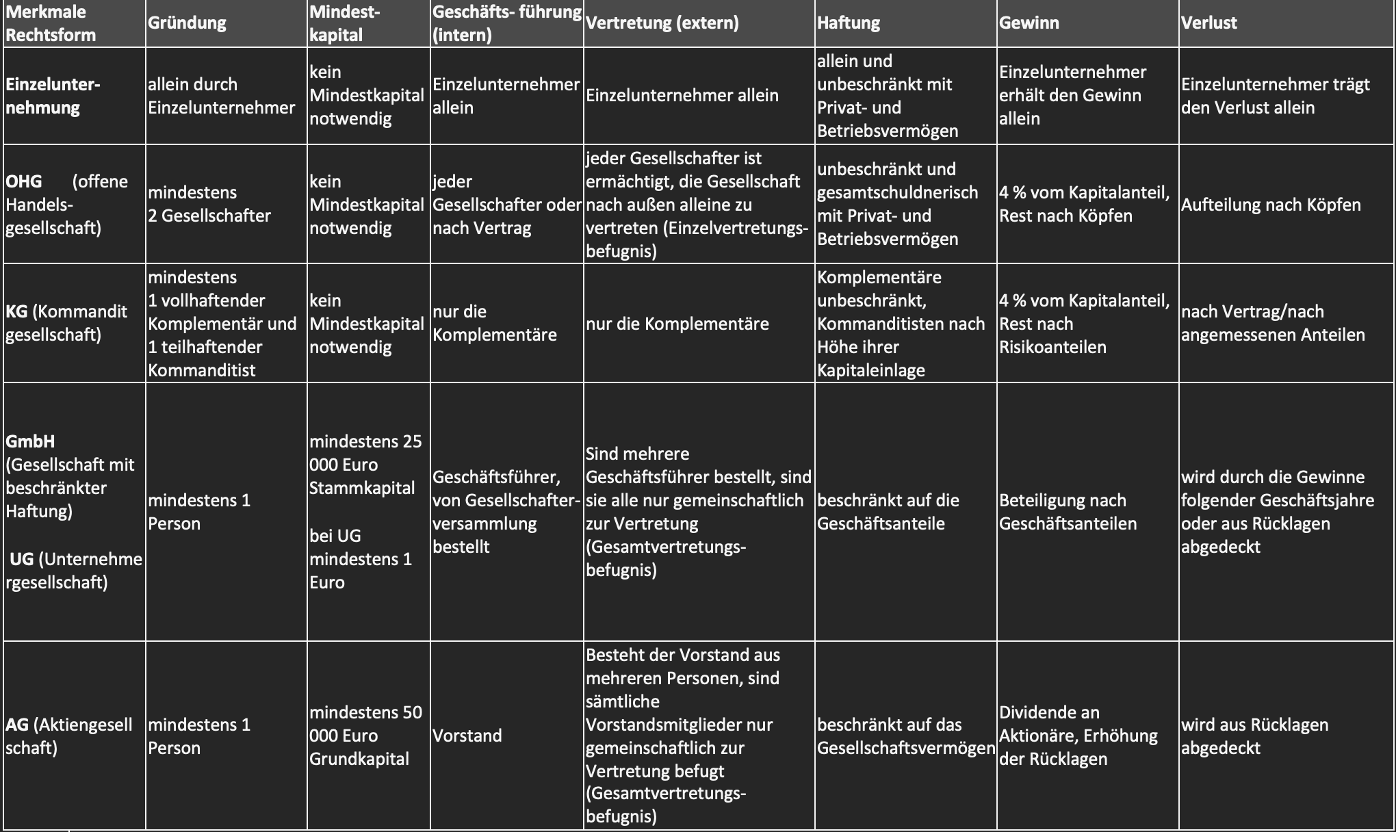
\includegraphics[height=9cm]{arten.png}
    \end{center}
    \caption{Arten von Firmen}
    \label{fig: Arten von Firmen}
\end{figure}

\subsubsection{Firmengrundsätze}
Firmen müssen folgende Grundsätze einhalten:
\begin{enumerate}
    \item \textbf{Firmenwahrheit und Firmenklarheit}: Die Firma darf nicht irreführend,  sprich klar und eindeutig sein. Es dürfen beim Kunden keine falschen Erwartungen entstehen.
    \item \textbf{Offenlegung der Gesellschaftsverhältnisse}: Diese Offenlegung beinhaltet Infos über Gesellschafter und Eigentümer als auch deren Anteile.
    \item \textbf{Offenlegung der Haftungsverhältnisse durch Rechtsformzusatz}: Eine Firma muss ihren Haftungsstatus klarstellen. Dies geschieht durch den Zusatz zur Firmenbezeichnung.
    \item \textbf{Firmenbeständigkeit}: Hier geht es darum, dass  der Name der nicht zu  oft wechseln darf und nur mit Begründung.
    \item \textbf{Firmenöffentlichkeit}:  Jedes Unternehmen muss im Handelsregister eingetragen sein.
    \item \textbf{Firmenausschließlichkeit}: Der Name einer Firma muss sich von den Namen aller anderen Firmen unterscheiden.
    \item \textbf{Firmengeheimnis}: Bestimmte Informationen dürfen geheim gehalten werden um wettbewerbsfähig zu bleiben.
    \item \textbf{Firmenfortführung}: Wird das Unternehmen  verkauft/in eine  andere Rechtsform umgewandelt, so bleibt die Bezeichnung i.d.R gleich. \\
          Dies soll das Vertrauen der Kunden und Geschäftspartner in das Unternehmen erhalten.
    \item \textbf{Firmenlöschung}: Wenn ein Unternehmen aufgelöst oder liquidiert wird, muss die Firmenbezeichnung aus dem Handelsregister gelöscht werden. \\
          Dies bedeutet, dass die Firma nicht mehr aktiv ist und keine Geschäfte mehr tätigt.
\end{enumerate}

\subsubsection{Grundfunktionsbereiche}

\begin{figure}[H]
    \begin{center}
        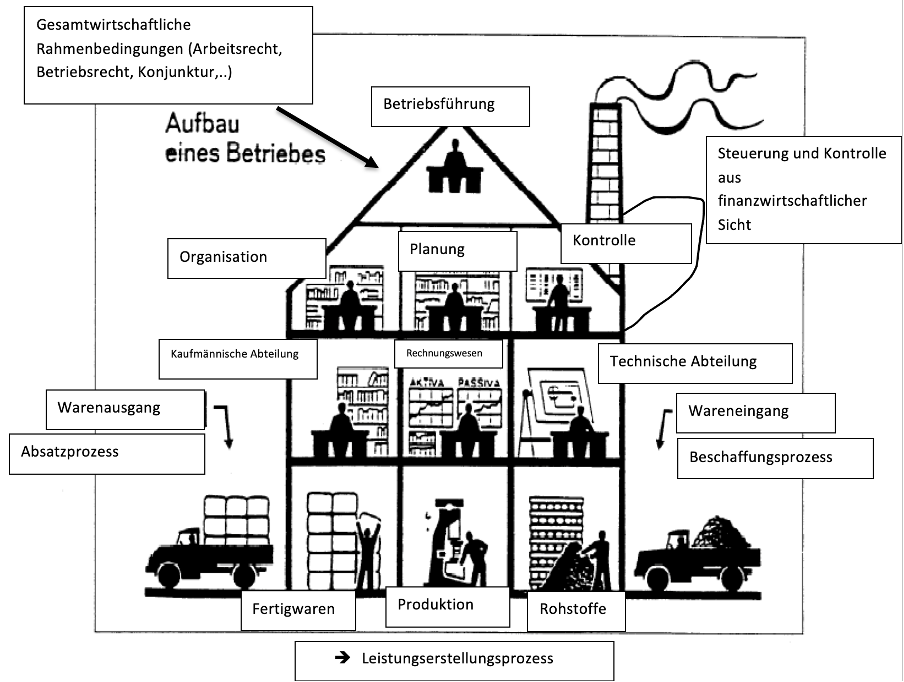
\includegraphics[height=6cm]{funktionsbereiche_firma.png}
    \end{center}
    \caption{Grundfunktionsbereiche von Firmen}
    \label{fig: Grundfunktionsbereiche von Firmen}
\end{figure}
Als Grundfunktionsbereich bezeichnet man Bereiche, die für Industriebetriebe charakteristisch/unverzichtbar sind. \\
Es wird in die folgenden Grundfunktionsbereiche unterschieden:
\begin{itemize}
    \item \textbf{Materialwirtschaft}: Beschaffung, Verwaltung von  Materialien
    \item \textbf{Produktionswirtschaft}: Organisiert die Fertigung
    \item \textbf{Absatzwirtschaft}: Dreht sich um den Verkauf des Produzierten
\end{itemize}

\subsubsection{Unterstützungsfunktionsbereiche}
Neben den Grundfunktionsbereichen gibt es noch die Unterstützungsfunktionsbereiche. \\
Diese sind dafür verantwortlich, dass die Grundfunktionsbereiche reibungslos ablaufen können. \\
Zu ihnen gehören:
\begin{itemize}
    \item \textbf{Finanzwirtschaft}: Dieser wird nochmal unterteilt in:
          \begin{itemize}
              \item \textbf{Finanzierung}: Bezeichnet die Bereitstellung finanzieller  Mittel.
              \item \textbf{Investition}: Bezeichnet die Verwendung finanzieller Mittel (größere  Beiträge, Kapitalbindung)
          \end{itemize}
    \item \textbf{Personalwirtschaft}: Beschäftigt sich mit Anzahl und Qualifikationen des Personals
    \item \textbf{Rechnungswesen}: Erfassung des  betrieblichen Prozesses eines Unternehmens. \\
          Man unterscheidet in:
          \begin{itemize}
              \item \textbf{Internes Rechnungswesen}:
                    \begin{itemize}
                        \item Kosten- und Leistungsrechnung
                        \item Betriebsstatistik
                        \item Planungsrechnung
                    \end{itemize}
              \item \textbf{Externes Rechnungswesen}:
                    \begin{itemize}
                        \item Buchführung
                        \item Jahresabschlussrechnung
                    \end{itemize}
          \end{itemize}
    \item \textbf{Controlling}: Das Controlling unterstützt die Geschäftsleitung indem es:
          \begin{itemize}
              \item Informationen beschafft \& aufbereitet
              \item das Unternehmen mitsteuert, koordiniert und analysiert
          \end{itemize}
\end{itemize}

\subsubsection{Querschnittsfunktion}
Die Unterstützungsfunktionsbereiche haben eine Querschnittsfunktion. \\
Diese besagt, dass die einzelnen Unterstützungsfunktionsbereiche jeweils allen Grundfunktionsbereichen zuarbeiten. \\
So regelt beispielsweise die Personalwirtschaft im Einvernehmen mit der Geschäftsleitung jeweils alle Personalentscheidungen, also sowohl in der Absatz- wie in der Produktions- oder Materialwirtschaft.

\begin{figure}[H]
    \begin{center}
        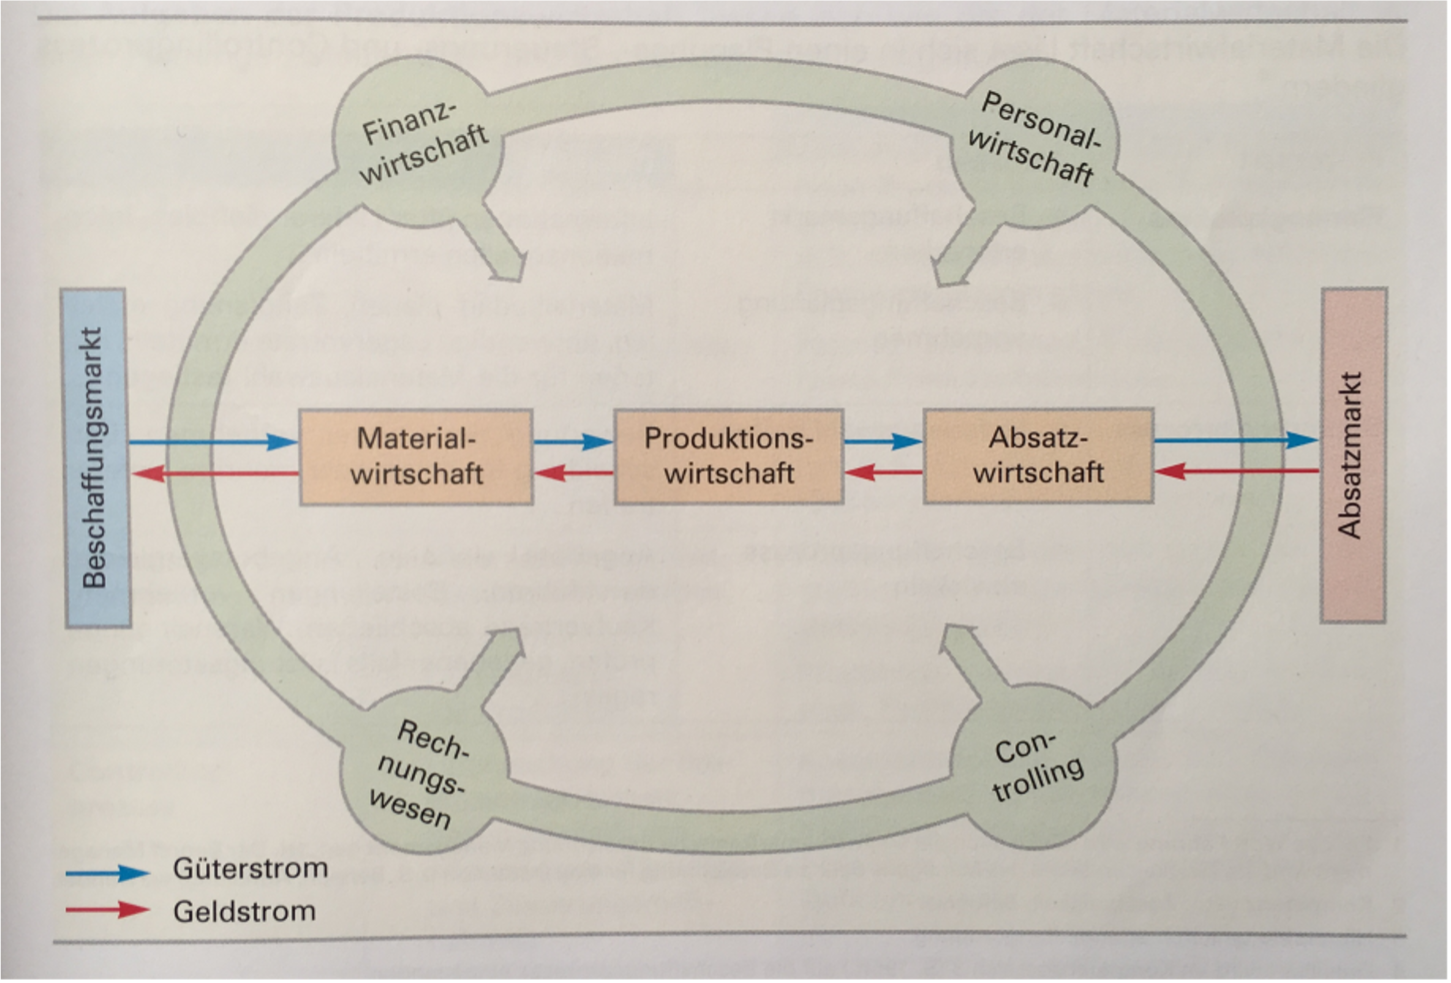
\includegraphics[height=6cm]{querschnitt.png}
    \end{center}
    \caption{Die Querschnittsfunktion}
    \label{fig: Die Querschnittsfunktion}
\end{figure}

\subsection{Prokura}
Eine Prokura ist eine Vollmacht, die eine Person oder mehrere Personen ermächtigt, im Namen eines Unternehmens oder einer Organisation rechtsgültige Entscheidungen zu treffen und Verträge abzuschließen. \\
Der Prokurist ist ein kaufmännischer Angestellter, dessen Wirkungsbereich im Interesse der Rechtssicherheit nach außen durch eine typisierte Vertretungsmacht festgelegt ist. \\ \\
Die Eintragung erfolgt durch den Kaufmann und nur mit ausdrücklicher Erklärung. \\
Eine deklaratorische HR-Eintragung ist notwendig. \\
Eine  Prokura ist im  Innenverhältnis mit Ernennung gültig, im Außenverhältnis erst  nach HR-Eintragung und Mitteilung an Dritte. \\
Der Umfang der Prokura kann nach \textbf{außen}  nicht beschränkt werden. \\ \\

\break

Beendet  wird  die  Prokura durch:
\begin{itemize}
    \item Auflösung des Arbeitsvertrages
    \item Widerruf
    \item Geschäftsauflösung
    \item Tod des Prokuristen
    \item \textbf{Nicht}  bei Tod des Geschäftsinhabers
    \item Bei Inhaberwechsel, wenn der neue Inhaber dies will
\end{itemize}


\subsubsection{Varianten}
\begin{itemize}
    \item \textbf{Einzelprokura}: Es gibt nur 1  Prokurist (höchste Prokura).
    \item \textbf{Filialprokura}: Prokurist hat nur über 1 Niederlassung Befugnisse.
    \item \textbf{Gesamtprokura}: Bestimmt mehrere Prokuristen (niedrigste Prokura)
\end{itemize}

\begin{figure}[H]
    \begin{center}
        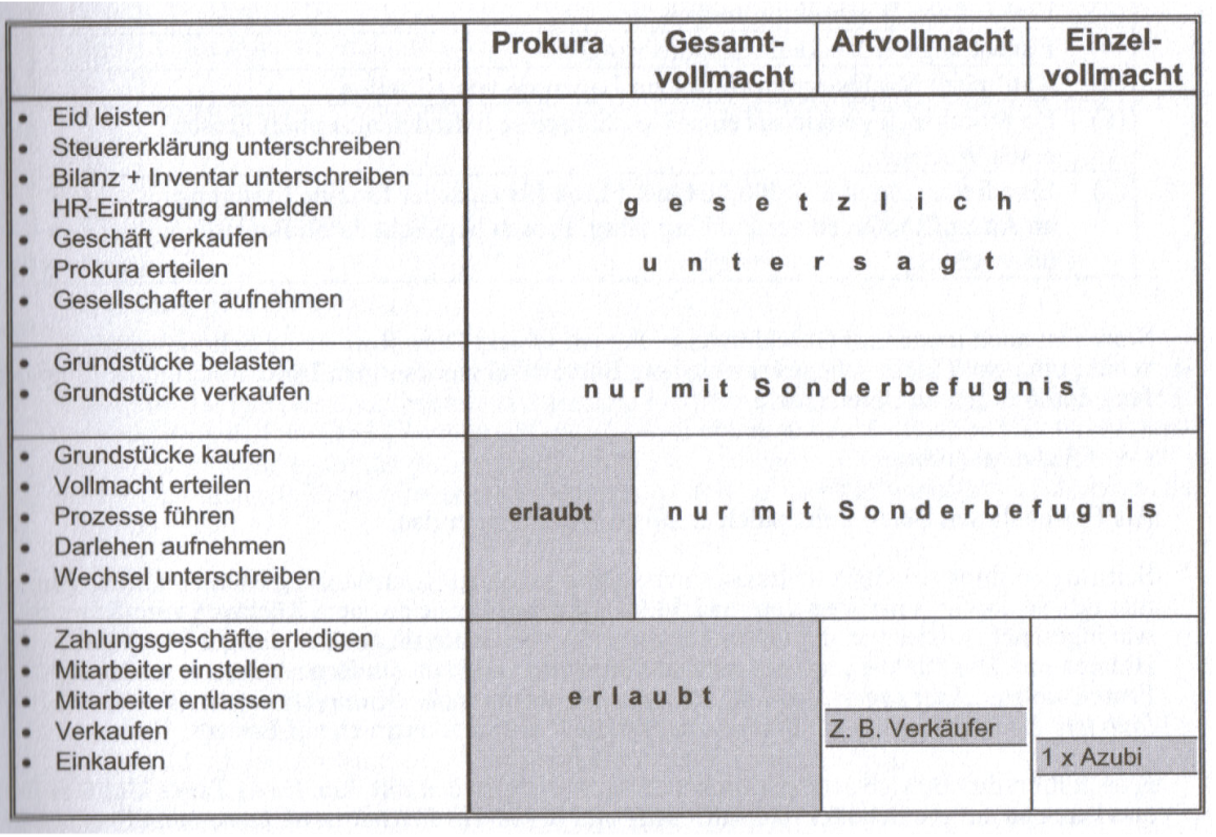
\includegraphics[height=6cm]{prokura.png}
    \end{center}
    \caption{Rechte der Prokuristen}
    \label{fig:Rechte der Prokuristen}
\end{figure}

\subsection{Handlungsvollmacht}
Es gibt verschiedene Varianten:
\begin{itemize}
    \item \textbf{Allgemeine Handlungsvollmacht}: Erlaubt, alle üblichen Aufgaben des Geschäftszweigs zu tätigen. Man unterscheidet ob mit Sondervollmacht oder ohne.
    \item \textbf{Artvollmacht}: Wahrnehmung begrenzter, sich wiederholender Aufgaben gleicher Art
    \item \textbf{Einzelvollmacht}:  Wahrnehmung einzelner Aufgaben
\end{itemize}
Die  Erteilung einer  Handlungsvollmacht  erfolgt durch:
\begin{itemize}
    \item den Kaufmann
    \item den Prokuristen
    \item einen weitgehend bevollmächtigten (`Untervollmachten`)
    \item Formlos
    \item Keine Eintragung notwendig
\end{itemize}
Sie kann widerrufen werden durch:
\begin{itemize}
    \item Widerruf
    \item Kündigung des Arbeitsvertrages
    \item Geschäftsauflösung
    \item Inhaberwechsel, wenn der Inhaber widerruft
    \item Einzelvollmacht
\end{itemize}

\subsection{Kaufmann}
Ein Kaufmann ist, nach dem Handelsgesetzbuch (HGB) der, der ein Handelsgewerbe betreibt. \\
Ein Handelsgewebe ist ein Gewerbe mit einer Kaufmännischen Organisation\\
(Eine Firma die Umsatz, Gewinn macht, Mitarbeiter hat, EDV-Anlagen == Firma die was verkauft) \\
Kaufmänner können unterschieden werden in:
\begin{itemize}
    \item Ist-Kaufmann
    \item Kann-Kaufmann
    \item Form-Kaufmann
\end{itemize}

\subsubsection{Ist-Kaufmann}
Ist-Kaufmann ist, wer ein Handelsgewerbe betreibt, das nach Art und Umfang einen kaufmännisch geführten Geschäftsbetrieb erfordert. \\
Der Inhaber eines solchen Geschäftsbetriebes ist kraft Gesetzes Kaufmann (Ist-Kaufmann). \\
Er muss sich in das Handelsregister eintragen lassen, ist jedoch schon vor Eintragung Kaufmann.

\subsubsection{Kann-Kaufmann}
Ein Kann-Kaufmann ist ein Kaufmann eines Kleingewerbes, der nicht im Handelsgesetzbuch eingetragen und somit nicht auf rechtlicher Grundlage ein Kaufmann ist. \\
Er wird zum Kaufmann im Sinne des HGB, sobald er im Handelsgesetzbuch eingetragen ist. \\ \\
Für Land und Forstwirtschaft gibt es hier eine Ausnahme: \\
Land und Forstwirtschaftliche Gewerbe mit einer kaufmännischen Einrichtung haben das Recht zur Eintragung. \\
Dadurch können sie zum kann-Kaufmann werden. \\
Ohne die kaufmännischen Organisation haben sie dieses Recht nicht und sind dadurch Nicht-Kaufmann.

\subsubsection{Form-Kaufmann}
Ein Formkaufmann besitzt die Kaufmannseigenschaft kraft seiner Rechtsform. \\
(z.b. GmbH, OHG, KG, etc.)

\subsection{Leitungssysteme}
Auch Weisungssysteme genannt. \\
Sie betrachten die Unternehmensstruktur unter dem Aspekt \"Uber- und Unterordnung (Weisungsbefugnis)

\subsubsection{Einliniensystem}
Kennzeichen: \\
\begin{itemize}
    \item Alle Mitarbeiter sind einer strengen Hierarchie gebunden
    \item Anweisungen erhält man immer von der Stelle unmittelbar \"uber der Eigenen
    \item Meldungen und Berichte gehen genauso nur an die Stelle darüber
    \item Nur dieser eine vertikale Dienstweg ist vorhanden und muss eingehalten werden
    \item Kontakte zu gleichrangigen Stellen führen zwingend über die gemeinsame übergeordnete Stelle
\end{itemize}
\begin{figure}[H]
    \begin{center}
        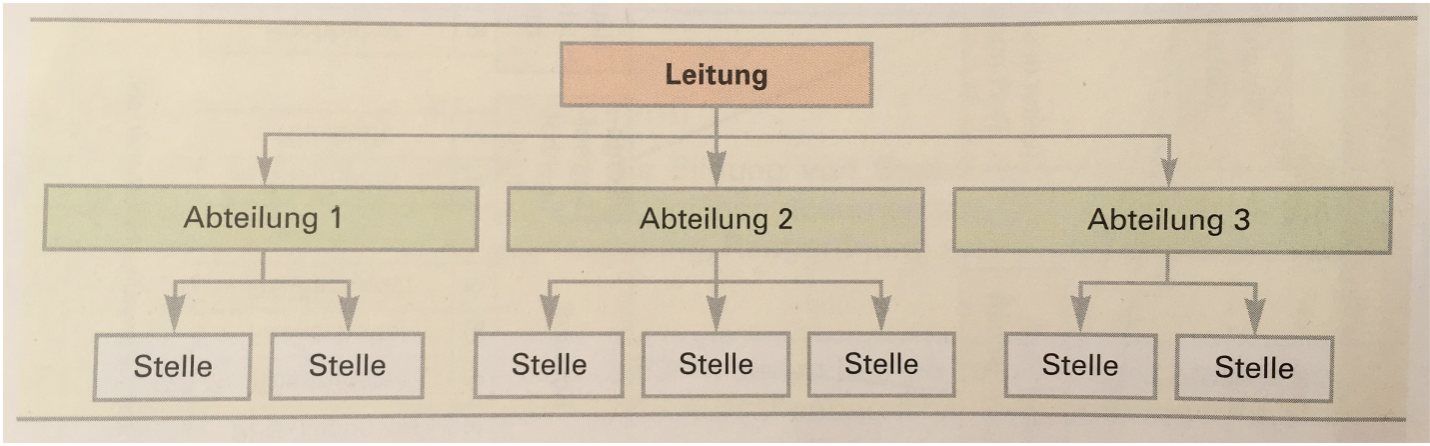
\includegraphics[height=6cm]{einlinien.png}
    \end{center}
    \caption{Einliniensystem}
    \label{fig:Einliniensystem}
\end{figure}
\textbf{Positives}:
\begin{itemize}
    \item \"Ubersichtlich
    \item Eindeutige und Abgegrenzte Dienstwege/Zust\"andigkeiten
    \item Keine Kompetenz\"uberschneidungen
    \item Starke Kontrollmöglichkeiten des Vorgesetzen nach unten
\end{itemize}
\textbf{Negatives}:
\begin{itemize}
    \item Überlastung der Führungsebene mit Routineaufgaben (Informationsweitergabe)
    \item Lange Dienstwege mit dem Risiko der Zeitverzögerung
    \item Bei Großunternehmen besteht das Risiko einer Überorganisation/Bürokratisierung
    \item Zwischeninstanzen können Informationen verfälschen oder unterdrücken
    \item Wenig Spielraum für eigenverantwortliches Handeln
\end{itemize}
\textbf{Fazit}:
Da mit zunehmender Betriebsgröße auch die Anzahl der Hierarchieebenen steigt, führt dies zunehmend zu Unüberschaubarkeit und langen Informationswegen. \\
Damit erhalten die Nachteile ein immer stärkeres Gewicht. \\
Die wenig wertschöpfenden Routineaufgaben binden mehr und mehr die kostbaren Ressourcen der Führungsebenen und die Unzufriedenheit der mündigen, aber eingeengten Mitarbeiter steigt. \\
Das Einliniensystem eignet sich daher nur für kleinere Betriebe.

\subsubsection{Mehrliniensystem}
Kennzeichen:
\begin{itemize}
    \item Ein Mitarbeiter kann von mehreren übergeordneten Vorgesetzten (Funktionsstellen) fachliche Anweisungen erhalten
    \item Im Gegensatz leitet er Berichte und Meldungen auch an die jeweilige übergeordnete Stelle zurück
\end{itemize}
\begin{figure}[H]
    \begin{center}
        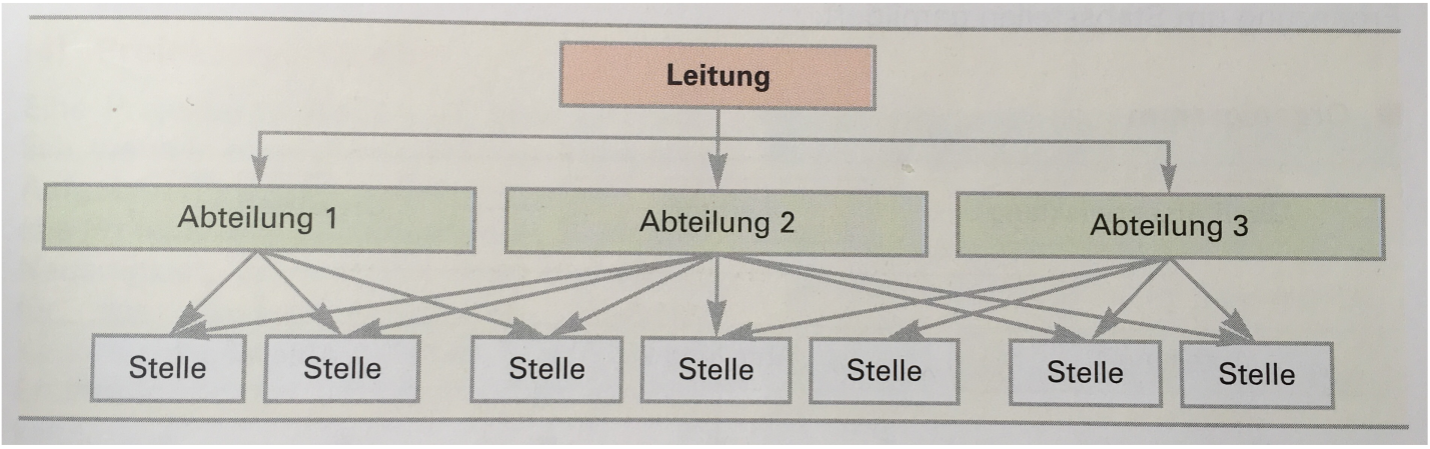
\includegraphics[height=6cm]{mehrlinien.png}
    \end{center}
    \caption{Mehrliniensystem}
    \label{fig:Mehrliniensystemm}
\end{figure}
\textbf{Positives}:
\begin{itemize}
    \item Entlastung der Führungsebenen von Routinearbeiten
    \item Instanzenwege werden verkürzt
    \item Die betrieblichen Hierarchien werden flacher
    \item Das Unternehmen kann flexibler reagieren
    \item Stelleninhaber können sich spezialisieren
\end{itemize}
\textbf{Negatives}:
\begin{itemize}
    \item Instanzenaufbau wird unübersichtlicher
    \item Erheblicher Abstimmungsaufwand
    \item Reibungsverluste, Verunsicherung und Überlastung des Stelleinhabers bei konkurrierenden statt kooperierenden Vorgesetzten
    \item Bei nicht klar abgegrenzten Kompetenzen besteht das Risiko von Konflikten
\end{itemize}
\textbf{Fazit}:
Mit zunehmender Betriebsgröße steigt die Komplexität der Gesamtaufgabe, sodass nur Spezialisten im Team diese Aufgaben bewältigen können. \\
Die Verkürzung der Instanzenwege durch ein fachliches Weisungsrecht in direktem Durchgriff entlastet von Routineaufgaben und erhöht damit die Effizienz des Gesamtsystems. \\
So hat z.B. der Ausbildungsleiter für alle Fragen der Berufsausbildung eine Weisungsbefugnis gegenüber allen Auszubildenden in den verschiedenen betrieblichen Aufgaben.

\subsubsection{Stabliniensystem}
Kennzeichen:
\begin{itemize}
    \item Die Stabstellen sind gegenüber den ihnen zugeordneten Leitungsstellen weisungsgebunden
    \item Stabstellen liegen außerhalb des Instanzenaufbaus
    \item Sie haben keine Weisungsbefugnis gegenüber den nachgeordneten Stellen, wohl aber ein Informationsrecht, wenn sie Auskünfte anderer Stellen zur Bewältigung ihrer Aufgabe benötigen
    \item Typische Aufgaben von Stabstellen: Beratung der Leitungsstelle, Begutachtung, Prüfung, Informationsbeschaffung und deren Auswertung, Entscheidungsvorbereitung, Erstellung von Richtlinien
    \item Beispiele: EDV, Organisation, Qualitätsentwicklung, Unternehmensplanung
\end{itemize}
\begin{figure}[H]
    \begin{center}
        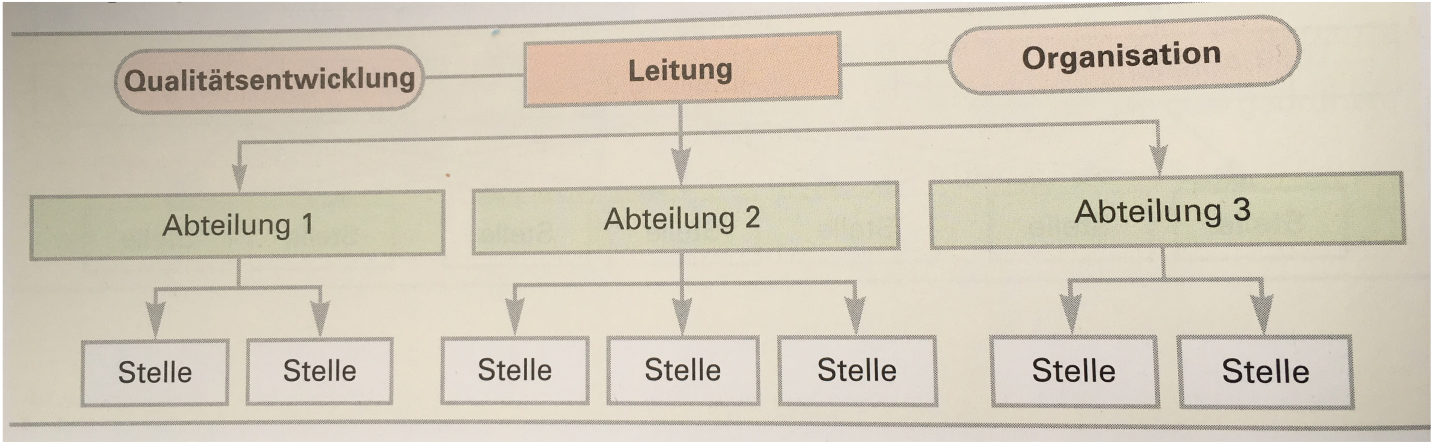
\includegraphics[width=12cm]{stablinien.png}
    \end{center}
    \caption{Stablinien}
    \label{fig:Stablinien}
\end{figure}
\textbf{Positives}:
\begin{itemize}
    \item Vorteile des Einliniensystems
    \item Die Entscheidungsbasis der Führungsebenen wird durch qualifizierte Stabstellen verbessert
    \item Nachwuchskräfte sammeln Erfahrung durch ihre Mitarbeit in verschiedenen Stabstellen
\end{itemize}
\textbf{Negatives}:
\begin{itemize}
    \item Grundprobleme des Einliniensystems werden nicht völlig beseitigt (z.B. lange Dienstwege)
    \item Personalkosten steigen durch teure Spezialisten in den Stäben
    \item Risiko, dass aufgrund der hohen fachlichen Kompetenz in den Stabstellen deren Einfluss auf die Geschäftsleitung sehr groß wird
    \item Liniensysteme können gute Vorschläge der Stabsstellen weiterhin unterbinden
\end{itemize}
\textbf{Fazit}:
Das Stabliniensystem bewahrt die Vorteile des Einliniensystems. \\
Es unterstützt die Geschäftsführung in der Qualität ihrer Entscheidungen wirkungsvoll durch die fachliche Kompetenz der Stäbe und vermeidet gleichzeitig die organisatorischen Risiken des Mehrliniensystems.

\subsection{Kritik an der Aufbauorganisation}
Die Aufbauorganisation führt zu Nachteilen, denn die Anstrengungen der einen Abteilung im Sinne des Gesamtunternehmens gewinnmaximierend zu handeln, kann den Anstrengungen der anderen Abteilungen zuwiderlaufen.
\begin{itemize}
    \item Gefahr, dass sich Mitarbeiter an mengenmäßiger Leistung orientieren, nicht an Kunden, Arbeitsqualität oder Termintreue
    \item Arbeitszerlegung fährt zu Tätigkeiten mit geringem Arbeitsinhalt, Monotonie und einseitiger Belastung. Selbstst\"andigkeit, Selbstverwirklichung k\"onnen weniger verwirklicht werden.
    \item i.d.R verlaufen betriebliche Prozesse "quer" zu den Funktionen
\end{itemize}

\subsection{Qualitätsmanagement}
Beinhaltet alle Maßnahmen zur
\begin{itemize}
    \item Planung
    \item Steuerung
    \item Optimierung
\end{itemize}
von Prozessen im Unternehmen. \\
Das Ziel ist es, eine bestimmte Qualität von Produkten /  Dienstleistungen zu erreichen. \\
Sie orientiert sich an Kundenwünschen, Meinungen und Feedback als auch messbaren  Merkmalen wie messbarer Qualit\"at.  \\
Die Produktqualität wird wie folgt gesichert:
\begin{itemize}
    \item Interne/Externe Audits
    \item \"Uberwachung von Prozessabl\"aufen
    \item Erstellung von Analysen und Reports
    \item Verantwortung für QM-Dokumentation
    \item Planung, Umsetzung und Weiterentwicklung des QM-Systems
    \item Mitarbeiter-Schulungen durchführen
\end{itemize}

\subsubsection{Total Quality Management (TQM)}
Es ist eine Erweiterung des traditionellen QM und schließt Mitarbeiter, Prozesse und Systeme mit ein. \\
Das Ziel ist es, eine Kultur der kontinuierlichen Verbesserung zu schaffen.

\subsubsection{Kontinuierlicher Verbesserungsprozess (KVP)}
Zentraler Bestandteil des QM. \\
Es geht darum, kontinuierlich Verbesserungen im Unternehmen zu erzielen, indem man Prozesse optimiert, Probleme l\"ost und Innovationen vorantreibt. \\
Der Fokus liegt auf der st\"andigen Weiterentwicklung und Verbesserung von Produkten, Dienstleistungen und Prozessen

\subsection{Quantitativer Angebotsvergleich / Handelskalkulation}
\label{sec:Handelskalkulation}
Damit ein Unternehmen Gewinne erzielen kann, müssen die Verkaufspreise so kalkuliert sein, dass sowohl die \textbf{Kosten gedeckt} werden, als auch eine \textbf{Gewinnspanne} einberechnet wird. Dies nennt man, außerhalb von Industrieunternehmen, \textbf{Handelskalkulation}. \\
Durch die folgenden Verfahren, können auch Preise für mehrere Angebote eines Produktes berechnet werden. Die Berechnung und den Vergleich dieser Preise nennt man \textbf{Quantitativer Angebotsvergleich}, da hier nur auf Basis des Preises verglichen wird.
\begin{figure}[H]
    \begin{center}
        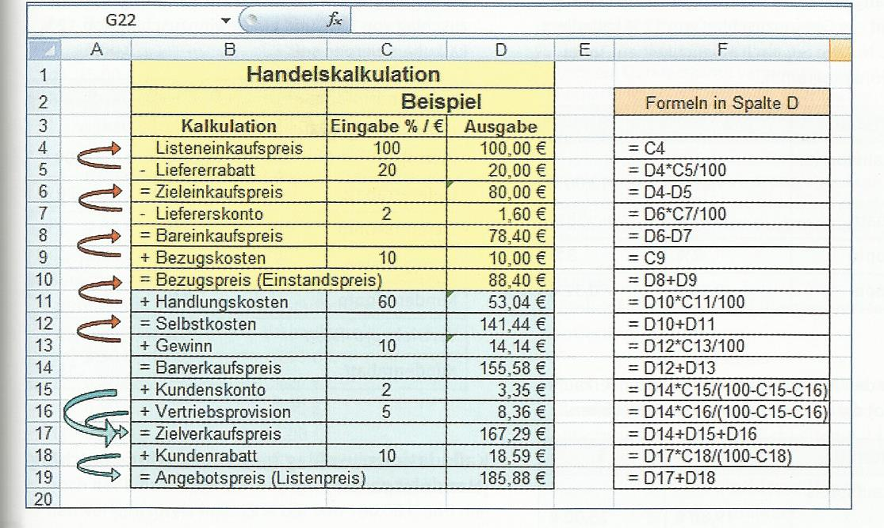
\includegraphics[height=6cm]{quantitativ.png}
    \end{center}
    \caption{Quantitativer Angebotsvergleich}
    \label{fig:Quantitativer Angebotsvergleich}
\end{figure}
Den gelben Teil nennt man auch \textbf{Bezugskalkulation}. \\
Der blaue Teil besteht aus der \textbf{Selbstkostenkalkulation} und \textbf{Absatzkalkulation}. \\ \\
Rechnet man vom Listeneinkaufspreis (oben) aus, so benutzt man die \textbf{Vorw\"artskalkulation}:
\begin{figure}[H]
    \begin{center}
        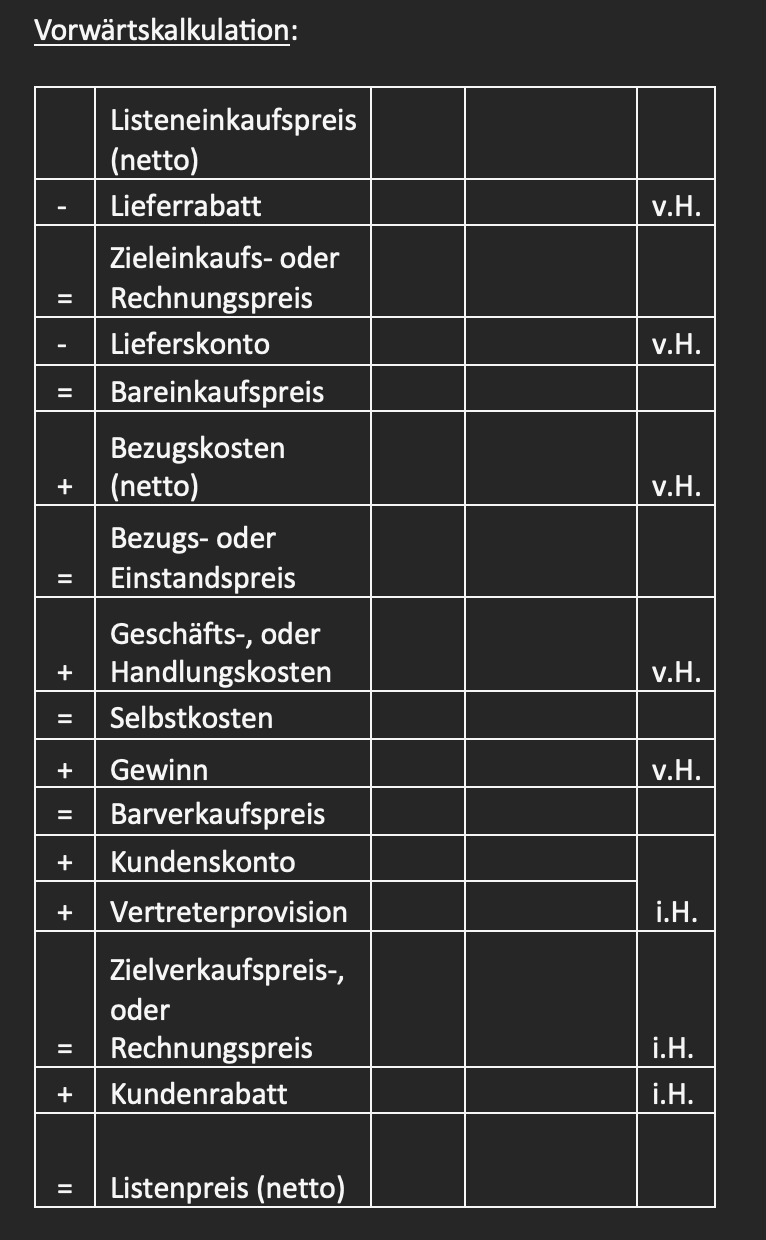
\includegraphics[height=12cm]{kalkV.png}
    \end{center}
    \caption{Vorwärtskalkulation}
    \label{fig:Vorwärtskalkulation}
\end{figure}
Hat man den Listenpreis (unten) gegeben, so benutzt man die \textbf{R\"uckw\"artskalkulation}
\begin{figure}[H]
    \begin{center}
        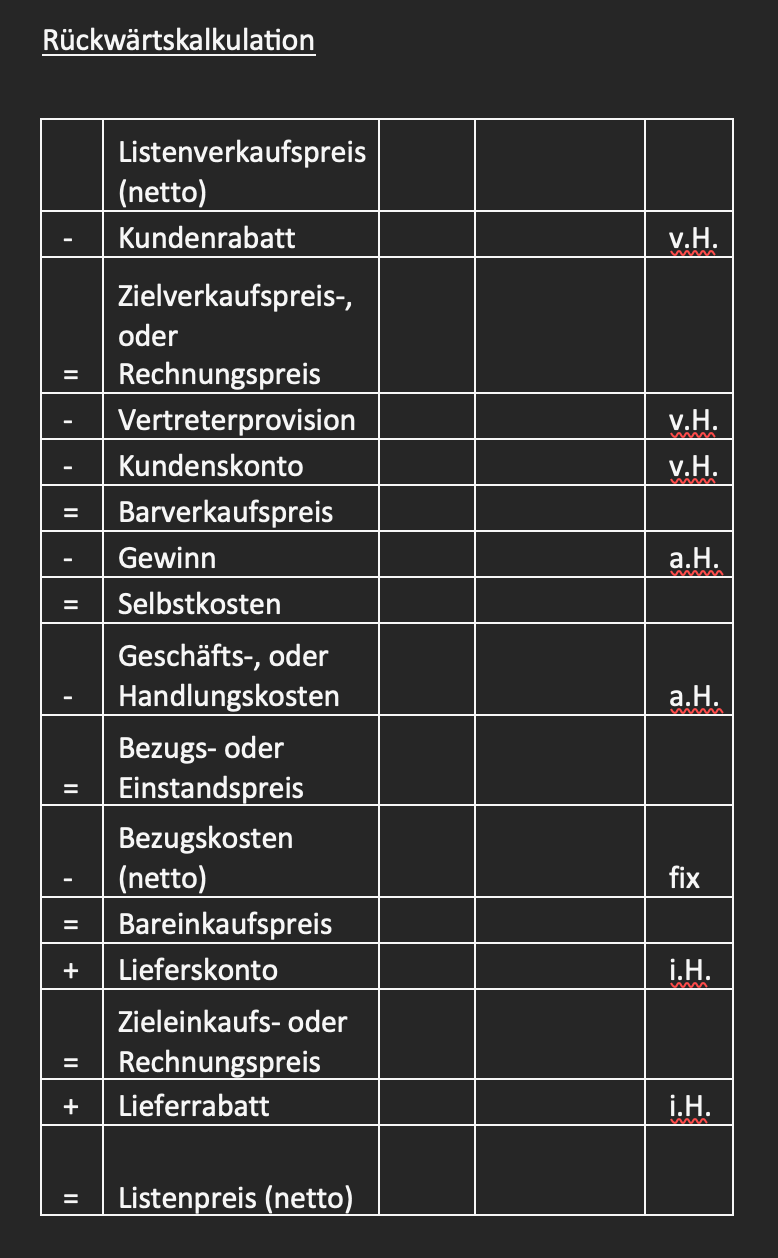
\includegraphics[height=12cmm]{kalkR.png}
    \end{center}
    \caption{Rückwärtskalkulation}
    \label{fig:Rückwärtskalkulation}
\end{figure}
Wenn man den Gewinn errechnen will, benutzt man die \textbf{Differenzkalkulation}:
\begin{figure}[H]
    \begin{center}
        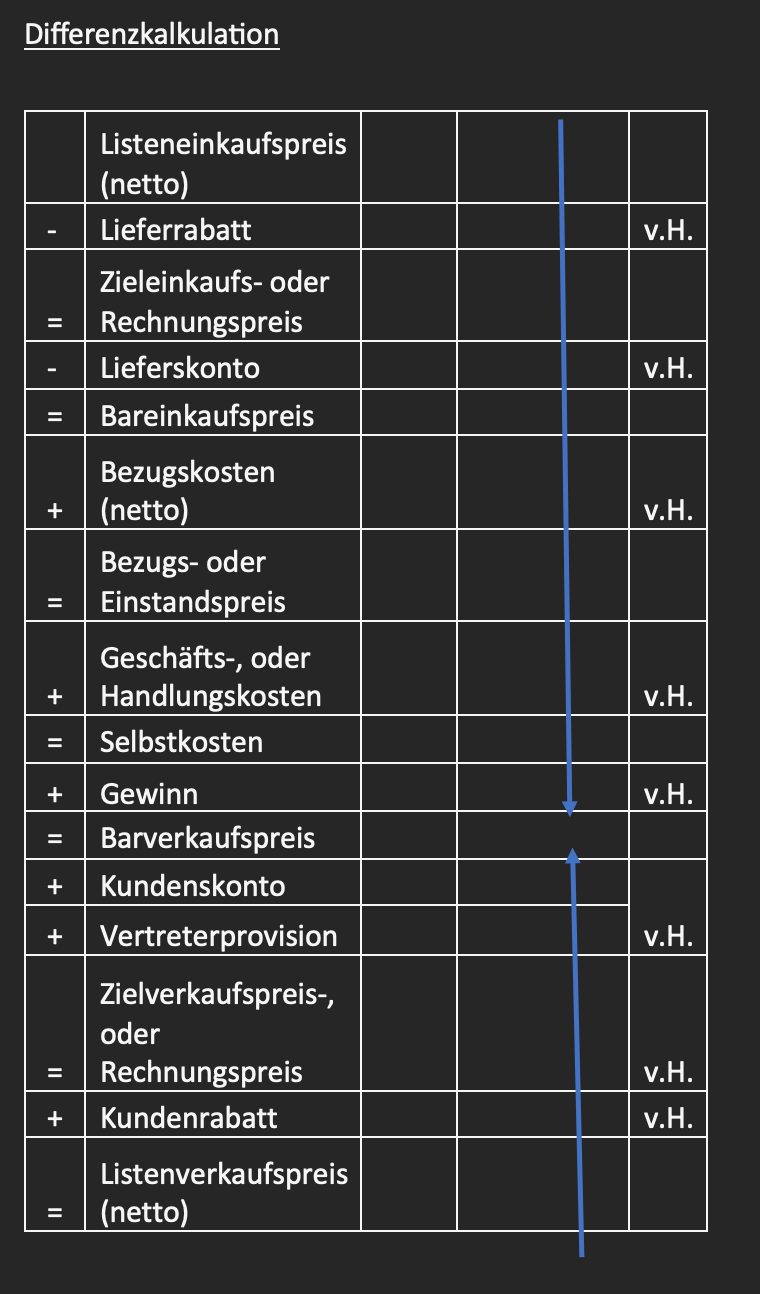
\includegraphics[height=12cm]{kalkD.png}
    \end{center}
    \caption{Differenzkalkulation}
    \label{fig:Differenzkalkulation}
\end{figure}
Um Zeit zu sparen kann man auch \textbf{verk\"urzte Kalkulationen} benutzen:
\begin{figure}[H]
    \begin{center}
        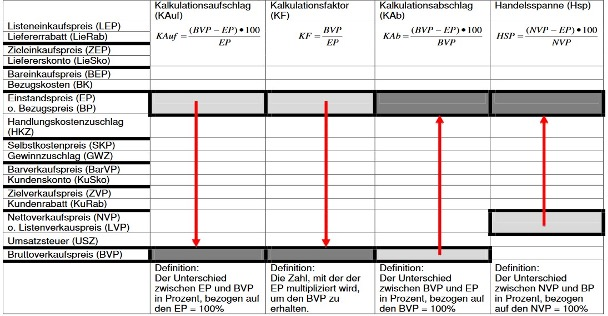
\includegraphics[width=12cm]{kalkS.jpg}
    \end{center}
    \caption{Verkürzte Kalkulation}
    \label{fig:Verkürzte Kalkulation}
\end{figure}

\break

\subsection{ABC-Analyse}

Die ABC-Analyse ist eine Methode zur Einteilung von Kunden, Produkten, Material und anderen Objekten in drei Klassen oder Kategorien: A, B oder C. \\
Die Objekte werden mit einer für die Analyse relevanten Kenngröße beschrieben und dann nach dieser Kenngröße sortiert. \\ \\
Schritt 1: $Menge * Preis$ \\
Schritt 2: Ordnen nach Preis in absteigender Reihenfolge \\
Schritt 3: Kumulativen Preis berechnen (vorherigen kumulativen Preis + Geradigen) \\
Schritt 4: Prozent ausrechnen (Prozent des kumulativen an der Stelle vom letzten \\ Kumulativen)
Schritt 5: Einteilen in Klassen
\begin{itemize}
    \item[A] bis inklusive 80\%
    \item[B] 81 bis inklusive 95\%
    \item[C] 96 bis 100\%
\end{itemize}
\begin{figure}[H]
    \begin{center}
        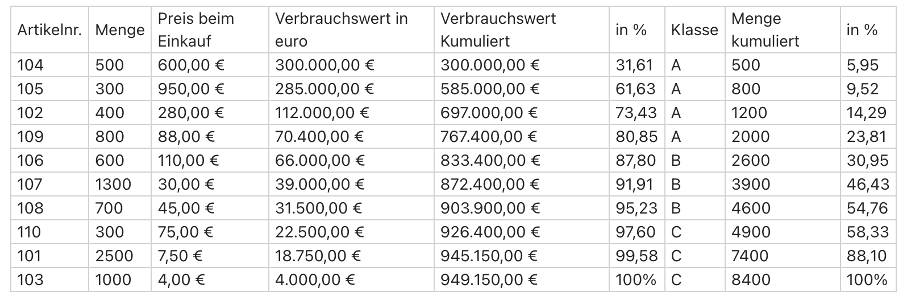
\includegraphics[width=12cm]{ABC.png}
    \end{center}
    \caption{ABC-Analyse}
\end{figure}

\subsection{Zahlungsverzug}
\begin{figure}[H]
    \begin{center}
        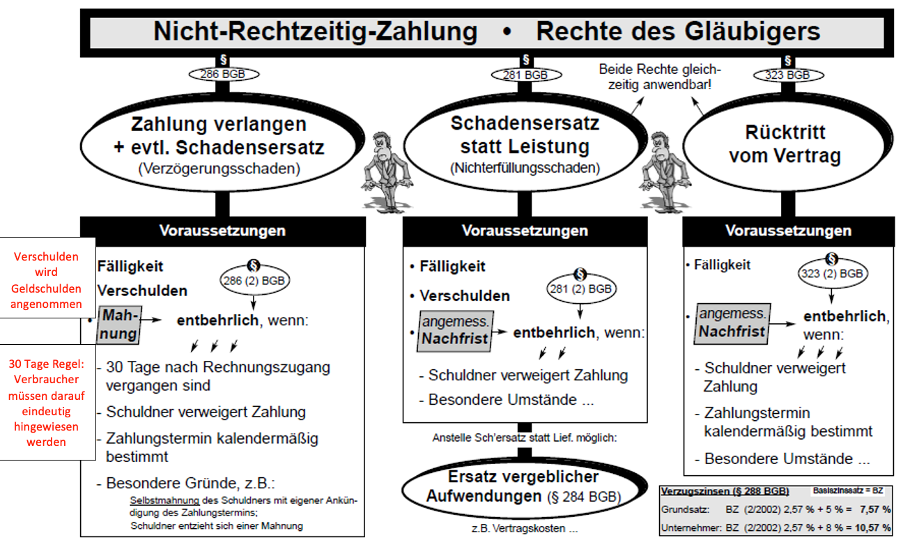
\includegraphics[width=12cm]{zahlungsverzug.png}
    \end{center}
    \caption{Zahlungsverzug}

\end{figure}
\subsubsection {Das außergerichtliche Mahnverfahren}
Gründe:
\begin{itemize}
    \item[-] gute Geschäftsbeziehungen nicht gefährden
    \item[-] Kunde könnte Zahlungstermin aus Versehen versäumt haben
\end{itemize}
\textbf {WICHTIG}: Rücksichtnahme ist hierbei schlecht, da eigene Zahlungsfähigkeit gefährdet wird

\subsubsection{Mahnstufen}
Mahnstufe 1 (3 Tage nach Fälligkeit) - höfliche Zahlungserinnerung\\
Mahnstufe 2 (nach 7 Tagen) – 1. Mahnungsbrief\\
Mahnstufe 3 (nach 7 Tagen) – 2. Mahnung mit Rechnungsdurchschrift und Zahlungsträger\\
Mahnstufe 4 (nach 7 Tagen) – 3. Mahnung mit Androhung d. Forderungseinzugs\\
Mahnstufe 5 (nach 7 Tagen) – Forderungseinzug\\
Mahnstufe 6 (nach 7 Tagen) – letzte Mahnung mit Androhung gerichtlichem\\
Mahnverfahren oder Klage\\
(hierbei keine Beachtung der 30-Tage-Frist)\\\textbf{}

\subsection{Beschaffung}
\subsubsection {Geschäftsprozess Beschaffung und Lagerhaltung}
\begin{figure}[H]
    \begin{center}
        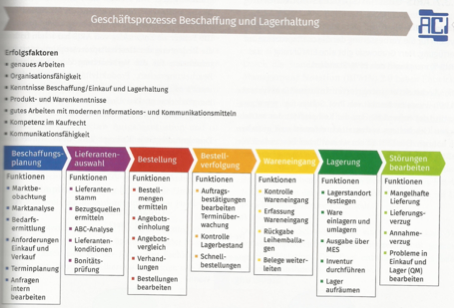
\includegraphics[width=12cm]{Beschaffung.png}
    \end{center}
    \caption{Zahlungsverzug}
\end{figure}

\subsubsection{Bedarfsermittlung}
\begin{itemize}
    \item[1.] Auftragsbezogene Bedarfsermittlung: \\
          Es wird der Bedarf anhand von konkreten Aufträgen und Stücklisten ermittelt, z.B. 100 Schränke, dafür werden 500m2 Holz benötigt.
    \item[2.] Verbrauchsorientierte Bedarfsermittlung: \\
          Es werden Vergangenheitswerte zugrunde gelegt, z.B. im Durchschnitt benötigen wir 300 Flaschen Holzkleber pro Jahr.
\end{itemize}

\subsubsection{Bestellverfahren}
\begin{itemize}
    \item[•]Feste Bestellmenge: Es wird immer die gleiche Menge bestellt.  \\ Geeignet für Güter mit gleichmäßigem Verbrauch, die eher günstiger im Einkauf sind
          \begin{itemize}
              \item[+] wenig Aufwand
              \item[+] kostengünstig
              \item[-] nicht flexibel (passt sich nicht an Schwankung an)
          \end{itemize}
    \item[•]Variable Bestellmenge: Termine können fest sein. \\
          Es wird immer genau die Menge bestellt, die gebraucht wird, geeignet für Güter mit Schwankungen in den Verkaufszahlen (z.B. saisonal bedingt) und höherpreisige Güter.
          \begin{itemize}
              \item[+]Immer die passende Menge auf Lager (nicht zu viel und nicht zu wenig)
          \end{itemize}
    \item[•]Optimale Bestellmenge: Summe aus Einstands-, Bestell- und Lagerkosten ist minimal
\end{itemize}

\subsubsection{Terminplanung}
\begin{itemize}
    \item[•]Bestellpunktverfahren: Meldebestand und Mindestbestand werden festgelegt.\\
          Menge kann fest oder variabel sein.
    \item[•]Bestellrhythmusverfahren: sich wiederholende, festgelegte Liefertermin.\\
          Man setzt hier meist die optimale Bestellmenge an.
    \item[•]Einzelbeschaffung
\end{itemize}

Probleme beim Bestellrhythmusverfahren: \\
überhöhte Lagerbestände oder Fehlmenge.n\\
Der durchschnittliche Lagerbestand sinkt wenn häufiger bestellt wird bzw. der Sicherheitsbestand niedriger angesetzt wird.

\subsubsection{Ermittlung der Bestellmenge}
Bestellpunktverfahren:
Es wird die Veränderung der Lagerbestände über einen gewissen Zeitraum überprüft, um die Bestellmenge optimal zu planen

\begin{figure}[H]
    \begin{center}
        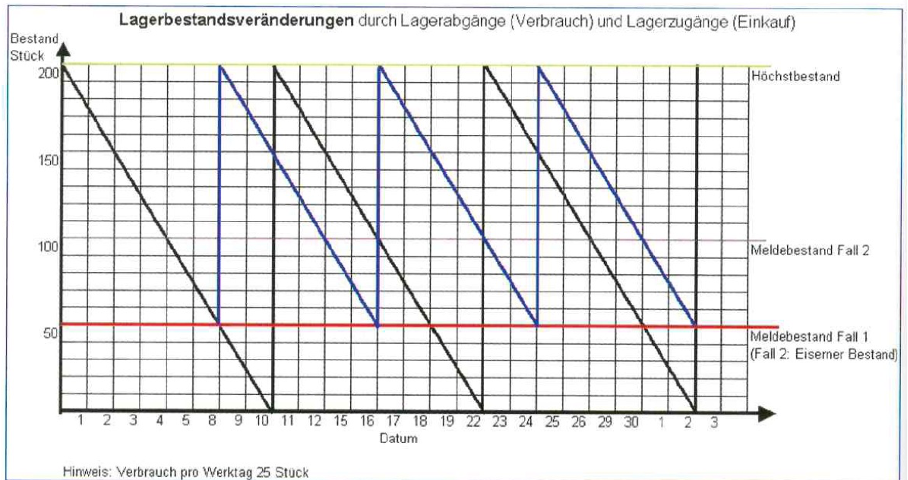
\includegraphics[width=12cm]{Lagerbestandveraenderungen.png}
    \end{center}
    \caption{Beispiel Lagerbestandver\"a"nderung}
    \label{fig:Lagerbestandveränderung}
\end{figure}

Das Schaubild zeigt die Lagerbestände eines Artikels. \\
Der Höchststand waren hier 200 Stück und einem regelmäßigen Verbrauch von 25 Stück pro Werktag. Der Bestand nimmt ständig ab und erreicht den Bestellpunkt/Meldebestand. Der Bestellpunkt ist der Zeitpunkt, zu dem bestellt wird während der Meldebestand die Menge ist, ab der  bestellt wird.\\
Die schwarze Kurve zeigt den Fall eines Meldebestandes von 50 Stück (Fall 1). Es werden dann 200 Stück bestellt, die nach zwei Tagen eintreffen, zum Punkt, an dem der Bestand auf 0 gesunken ist.
Im zweiten Fall (blaue Kurve) gibt es einen Sicherheitsbestand von 50 Stück und der Meldebestand beträgt jetzt 100 Stück. Wird der Höchstbestand beibehalten, muss jetzt häufiger in kleinerer Menge bestellt werden.


\begin{itemize}
    \item[1.]Durchschnittlicher Lagerbestand:
    \item[]Anfangsbestand = Mindestbestand + Bestellmenge
    \item[]Endbestand = Mindestbestand
    \item[]Durchschnittlicher Lagerbestand = (Anfangsbestand + Endbestand) / 2
    \item[]Oder Monatsgenaue Berechnung:
    \item[]Durchschnittlicher Lagerbestand = (Anfangsbestand + 12 * Monatsendbestände) / 13

    \item[2.]	Höchstbestand = Mindestbestand + optimale Bestellmenge
    \item[3.]	Meldebestand = Mindestbestand + (Tagesverbrauch * Lieferzeit)                 \item[]Stellt sicher, dass rechtzeitig bestellt wird (Beschaffungszeit wird überbrückt, Sicherheitsbestand wird nicht unterschritten)
    \item[4.]	Mindestbestand oder Sicherheitsbestand: eiserne Reserve, wird von der Geschäftsleitung festgelegt, darf nur in Ausnahmefällen unterschritten werden; soll Bedarfsunsicherheit, Lieferzeitunsicherheit und Bestandsunsicherheit abdecken

\end{itemize}

\subsubsection{Bestellrhytmusverfahren}
Das Bestellrhythmusverfahren ist eine Strategie, die ein Unternehmen innerhalb der Lagerverwaltung verfolgt. Ziel des Bestellrhythmusverfahrens ist es, den optimalen Zeitpunkt und die optimale Menge für die Materialbeschaffung festzulegen. Die zentralen Kennzahlen im Bestellrhythmusverfahren sind die optimale Bestellmenge und die Fehlmengenkosten.

\begin{figure}[H]
    \begin{center}
        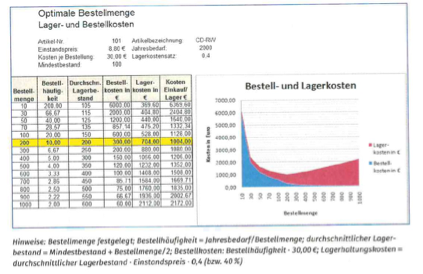
\includegraphics[width=12cm]{Bestellrhymusverfahren.png}
    \end{center}
    \caption{Beispiel Bestellrhytmusverfahren}
    \label{fig:my_label}
\end{figure}

\subsubsection{Eigenfertigung oder Fremdbezug (make or buy)?}
Man vergleicht bei freier Kapazität die Kosten bei Fremdbezug = Einstandspreis mit den variablen Herstellkosten bei Eigenfertigung. \\
Beispiel: Ein Industriebetrieb verkauft 7 verschiedene Produkte. Die Produkte 1 bis 5 werden im eigenen Unternehmen hergestellt.
Die Produkte 6 und 7 werden eingekauft und als Handelsware wieder verkauft.
Es ist Produktionskapazität frei.

\begin{figure}[H]
    \begin{center}
        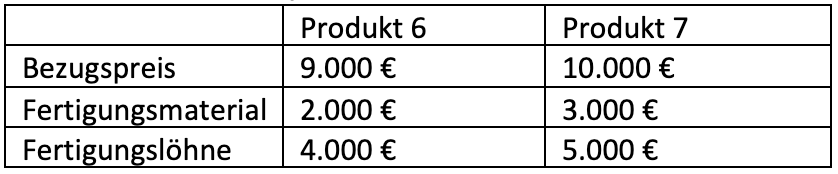
\includegraphics[width=12cm]{makeOrBuy.png}
    \end{center}
    \caption{Tabelle von Produkt 6 und 7}
    \label{fig:MakeOrBuy.png}
\end{figure}

\textbf{Materialgemeinkostenzuschlagssatz}: 25\%, davon 20\% variable Kosten./
Fix Kosten: unabhängig von der verkauften oder produzierten Menge z.B. Miete für Lagerräume/
Var. Kosten: ändern sich mit der verkauften oder produzierten Menge z.B. Stromkosten/
Fertigungsgemeinkostenzuschlagssatz: 120\%, davon 40\% variable Kosten.

\begin{figure}[H]
    \begin{center}
        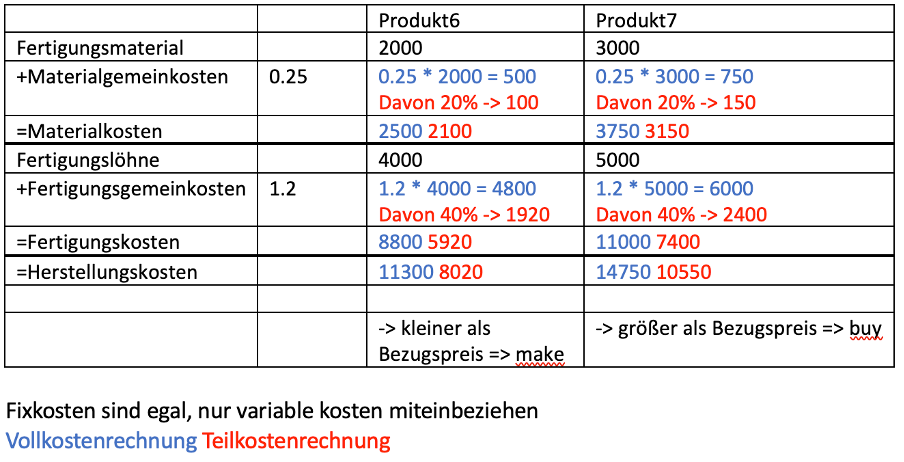
\includegraphics[width=12cm]{berechnungMakeOrBuy.png}
    \end{center}
    \caption{Tabelle zur Berechnung von Produkt 6 und 7}
    \label{fig:berechnungMakeOrBuy.png}
\end{figure}

\subsection{Kaufvertrag}
Verkäufer verpflichtet sich die Ware mangelfrei an den Käufer zu geben. Dabei zahlt man nur für die Sache/Produkt.
Sonderform: Verbrauchsgüterkauf (Unternehmen verkauft an Verbraucher)/
Fernabsatzvertrag (Unternehmen verkauft an Verbraucher fernmündlich z.B. Online Shopping)

\subsection{Werkvertrag}
Auftragsnehmer(Werkunternehmer) verpflichtet sich ein konkretes Werk zu erstellen oder zu liefern  (z.B. Erstellung einer Software ). Bei offensichtlichen Mängel \textrightarrow\space Notierung ins Abnahmeprotokoll, bei schweren Mängel \textrightarrow\space Verweigerung der Abnahme möglich.

\begin{itemize}
    \item[-] Der Gegenstand wird speziell nach Kundenwunsch angefertigt
    \item[-]Der Verkäufer muss einen mangelfreien Gegenstand übergeben (Verjährungsfrist bei Mängeln: 3 Jahre)
          \begin{itemize}
              \item Ist dies nicht der Fall muss der Verkäufer nachbessern bis der Mangel beseitigt ist (Die Kosten hierfür trägt der Verkäufer)
          \end{itemize}

\end{itemize}

Abnahmeerklärung (s.u. Ende des Beschaffungsprozesses): Erklärung, dass eine Sache bestimmten Kriterien entspricht. Auftraggeber erklärt sein Einverständnis oder Ablehnung des vom Auftragsnehmer erstellten Werkes (ggf. Mängelanzeige)

Leistungen aus einem Werkvertrag: §640 BGB; Unternehmen hat Anspruch auf die Abnahme
Problem: wesentlicher Mangel, dann keine Abnahme; oft fiktive Abnahme; Folgen: Vergütung wird fällig, Gefahr der zufälligen Verschlechterung geht auf den Besteller über, nur bei Abnahme aufgenommene Mängel müssen beseitigt werden, Verjährung beginnt

Dienstvertrag: § 611 BGB, Dienst wird geschuldet, keine Abnahme, =Arbeitsvertrag, es gelten Kündigungsvorschriften


\subsection{Dienstleistungsvertrag} Eine Person oder ein Unternehmen erbringt eine Dienstleistung für eine andere Person oder ein anderes/gleiches Unternehmen (z.B. IT Support).\
Der Unterschied zwischen einem Werksvertrag und einem Dienstleistungsvertrag ist, dass ein Werksvertrag genaue und konkrete Anforderungen hat (z.B. App soll eine Filter Funktion erhalten). Der Dienstleistungsvertrag fokussiert sich eher auf die Dienstleistung/Service (IT Support: Laptop soll funktionieren)\\
Sonderform: Arbeitsvertrag
\begin{itemize}
    \item[-] Hier wird ein Dienst also Arbeitszeit gekauft
    \item[-]Es wird die Arbeitszeit bezahlt, die auch benötigt wird (d.h. wenn unerwartete Probleme auftreten/der Kunde nicht zufrieden ist oder man länger braucht, wird auch diese Zeit bezahlt)
\end{itemize}

Dienstleistungsverträge im IT-Bereich:\
\begin{itemize}
    \item[-]IT-Sourcing: Dienstleistungen werden von extern beschafft
    \item[-]IT-Outsourcing: unbefristete Auslagerung von IT-Aufgaben, IT-Abteilungen, IT-Bereichen mit Vertrag (auch nur selektiv möglich)
    \item[-]Managed-Services: befristete Erledigung der Dienstleistungen durch externes IT-Systemhaus, mit Rahmenvertrag
    \item[-]Desktop-Services: Hard- und Software werden bereitgestellt, erneuert und gewartet
    \item[-]User-Helpdesk: Betreuung der Anwender im Unternehmen
    \item[-]Cloud-Services: Infrastruktur, Plattform oder Software werden vom Dienstleister bereitgestellt
    \item[-]Application Service Providing: über eine Datenleitung werden Anwendungen bereitgestellt, z.B. ERP-System
    \item[-]On-Side-Management: Übernahme von Funktionen in den Räumen des Kunden, teilweise oder vollständig mit Betriebsmitteln des Kunden
\end{itemize}

\break

IT-Servicearten:
\begin{itemize}
    \item[-]IT-Vertrieb, IT-Handel: Beschaffung von IT-Systemen und Komponenten, auch mit Aufbau und Anschluss an das vorhandene Netzwerk
    \item[-]Break oder Fix-Support, Field Service, Vor-Ort-Service: Ausführung von IT-Dienstleistungen von Technikern vor Ort, Arbeitszeit+Anfahrtskosten+Teile werden in Rechnung gestellt
    \item[-]Swap-Service: identisches Gerät wird als Ersatz zur Verfügung gestellt
    \item[-]DIY-Service: Do-It-Yourself-Service, Kunde darf Servicearbeiten selbst durchführen (Gewährleistung bleibt)
    \item[-]Live-Chat: über App oder ein Widget wird ein Chat-Kontakt zu einem Mitarbeiter hergestellt
    \item[-]Garantieservice: unentgeltlich aufgrund von Gewährleistung oder Garantie
    \item[-]IT-Einweisung, IT-Training, IT-Schulung
    \item[-]Serviceverfügbarkeit
    \item[-]Serviceportfolio, Servicekatalog
\end{itemize}


\begin{figure}[H]
    \begin{center}
        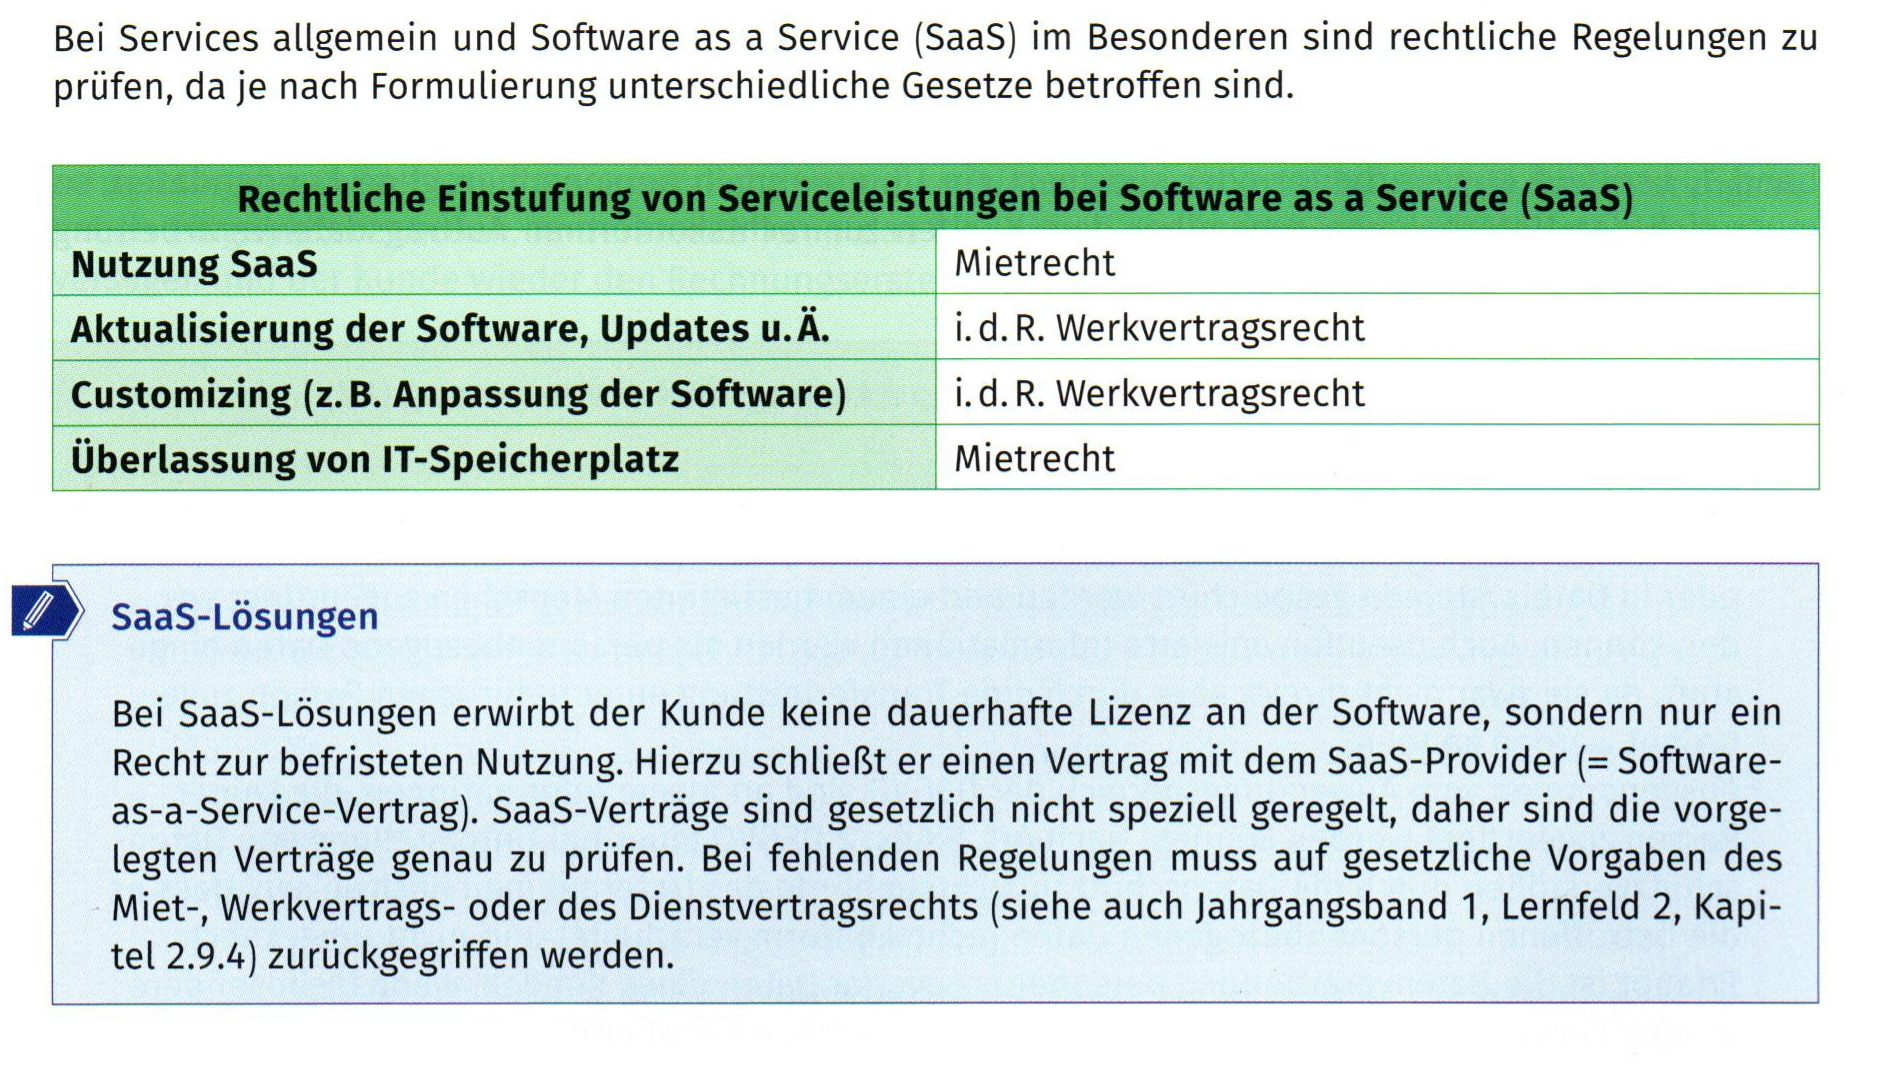
\includegraphics[width=12cm]{SaaS1.png}
    \end{center}
    \label{fig:saas1.png}
\end{figure}

\begin{figure}[H]
    \begin{center}
        \includegraphics[width=12cm]{SaaS2.png}
    \end{center}
    \label{fig:saas2.png}
\end{figure}

\begin{figure}[H]
    \begin{center}
        \includegraphics[width=12cm]{IT_Service.png}
    \end{center}

    \label{fig:IT_Service.png}
\end{figure}

\subsection{Ablauf eines Kaufvertrages}

\begin{figure}[H]
    \begin{center}
        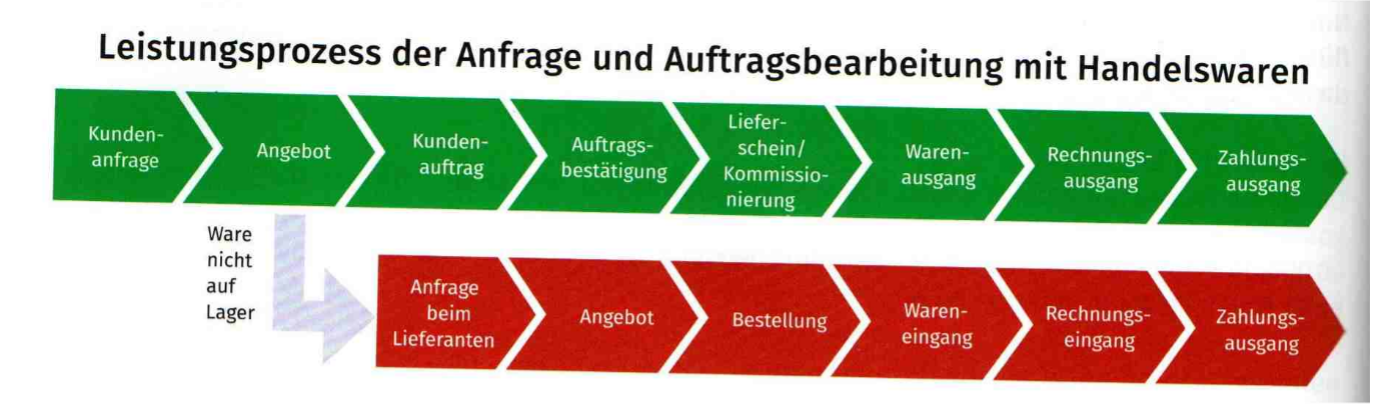
\includegraphics[width=12cm]{Kaufvertragablauf.png}
    \end{center}
\end{figure}

\begin{figure}[H]
    \begin{center}
        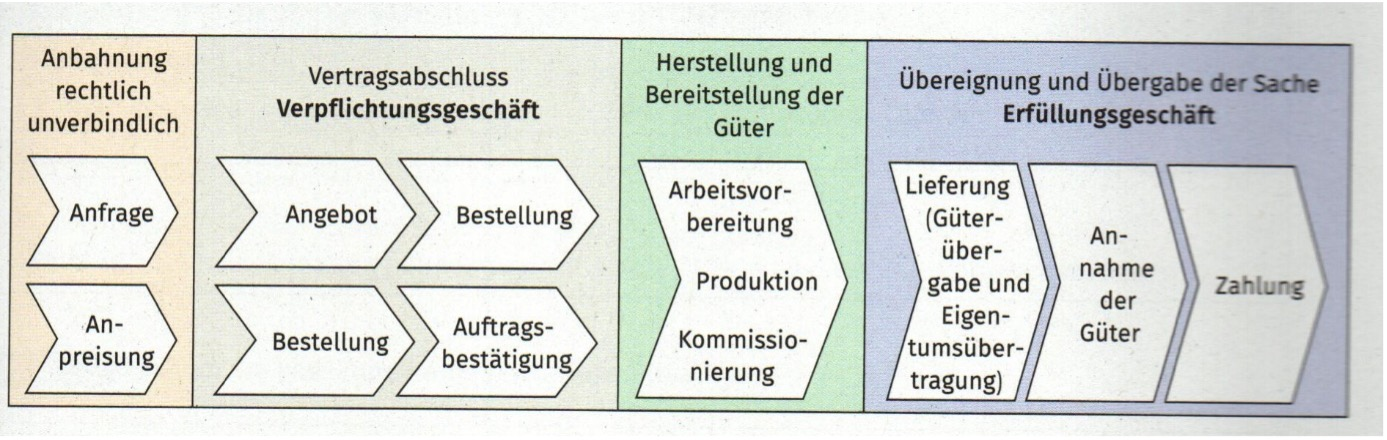
\includegraphics[width=12cm]{Kaufvertragablauf2.jpg}
    \end{center}
\end{figure}

\subsection{Angebotsvergleich}
\begin{figure}[H]
    \begin{center}
        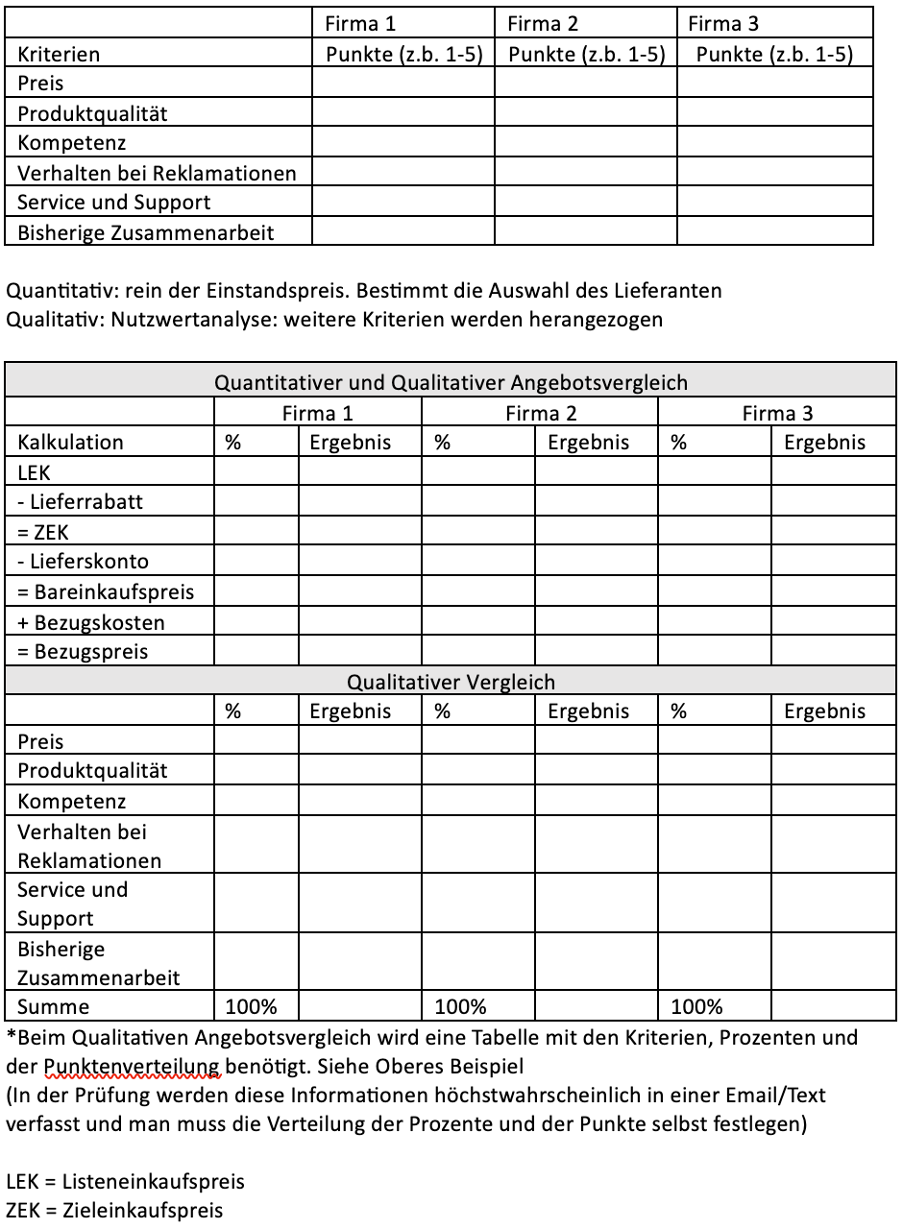
\includegraphics[width=12cm]{QuantitativUndQualitativerAngebotsvergleich.png}
    \end{center}
    \label{fig:QuantitativUndQualitativerAngebotsvergleich.png}
\end{figure}

\subsection{Ende des Beschaffungsprozesses}
(Wareneingang bzw. Abnahme der Leistung)

Ist die Warenlieferung im Eingangslager angekommen, wird sie geprüft, mit den Lieferpapieren verglichen und der Lagereingang im Computer erfasst. Durch elektronische Datenerfassung und Datenübertragung werden die Lieferdaten von den Lieferpapieren oder Verpackungen schnell aufgenommen, abgeglichen und dokumentiert. Bei einem Mangel wird eine Mängelanzeige im System oder auf einem Formular erstellt:

\begin{figure}[H]
    \begin{center}
        \includegraphics[width=12cm]{Mängelanzeige.png}
    \end{center}
    \caption{Mängelanzeige}
    \label{fig:Mängelanzeige.png}
\end{figure}

Ist alles in Ordnung, wird die Lieferung im Vorratslager an den richtigen Platz gebracht, ansonsten häufig ein Platz in einem Zwischenlager gesucht. Ein weiterer wichtiger Arbeitsbereich im Lager ist das Ausgangs- oder Kommissionierungslager. Hier werden entsprechend dem Lieferschein oder Auftrag die Waren für den Kunden zusammengestellt, die verschiedenen Packstücke zu einer Ladeeinheit zusammengefasst und mit den Lieferpapieren für Kunden bestückt. Wenn die Lieferung vom Lieferanten schon für die Weiterlieferung an den Kunden verpackt wurde, wird sie gleich in das Ausgangslager gebracht. Bei der Warenannahme wird in zwei Schritten vorgegangen:

Äußerliche Sichtkontrolle in Anwesenheit des Überbringers und später eine genauere Kontrolle der Lieferung. Material- und Warenlieferungen müssen unverzüglich überprüft werden.

\begin{figure}[H]
    \begin{center}
        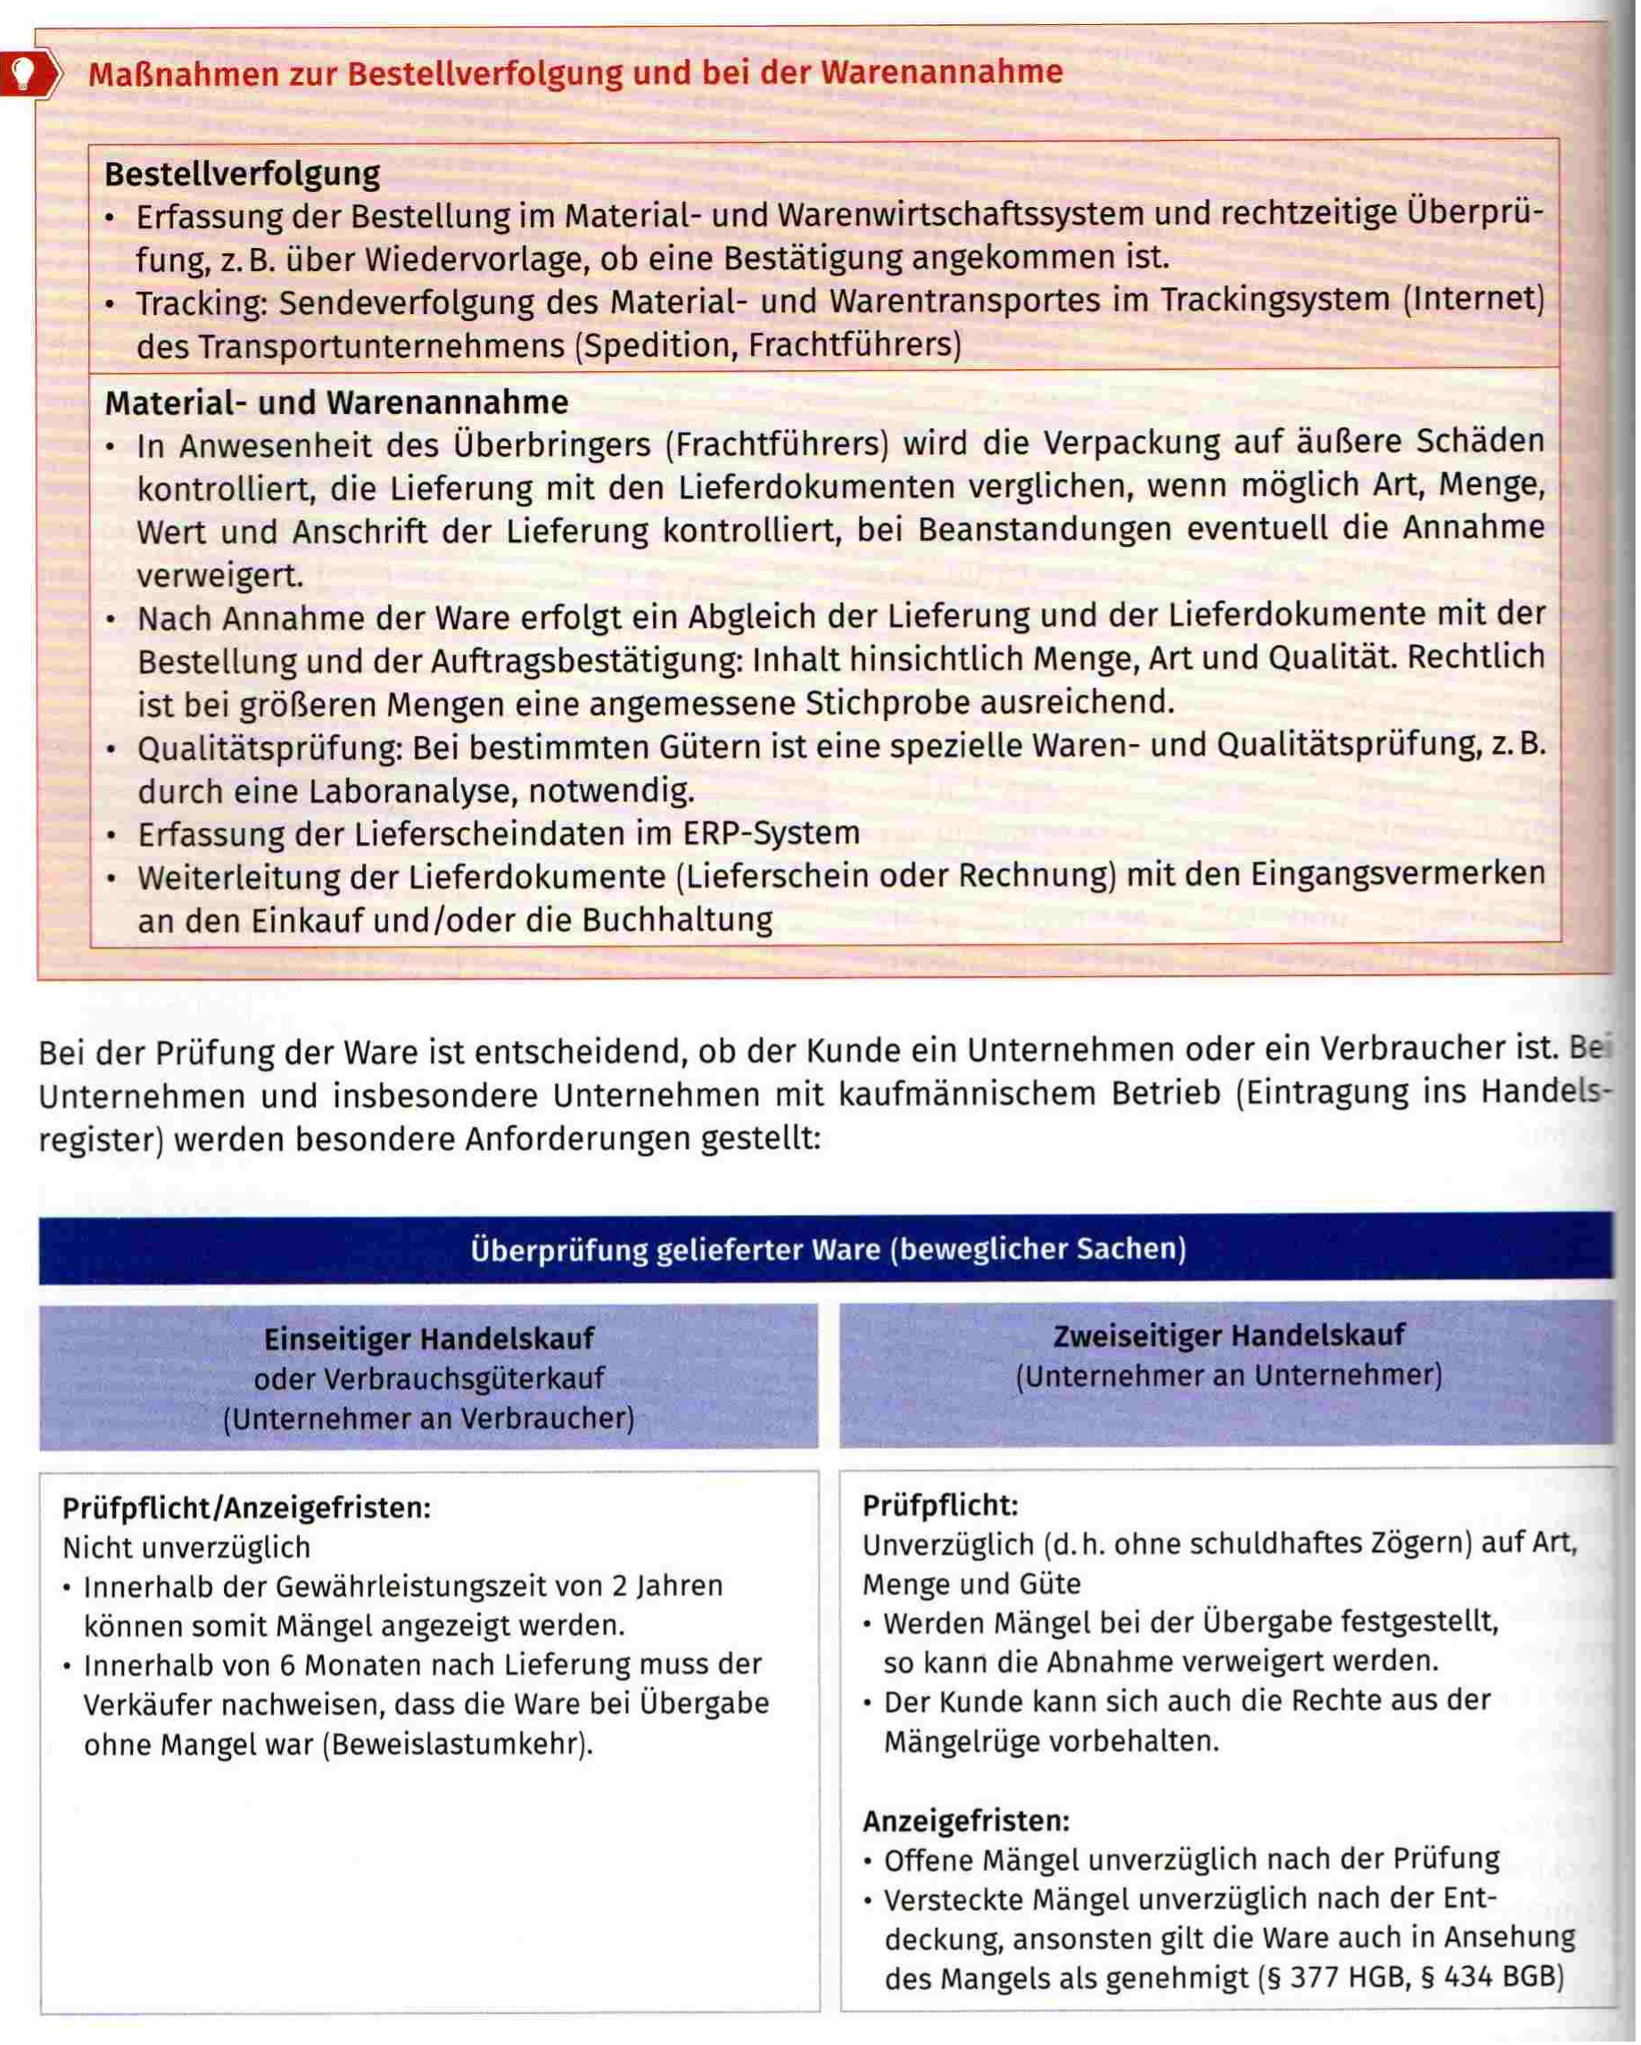
\includegraphics[width=12cm]{überprüfungWarenanahme.png}
    \end{center}
    \label{fig:überprüfungWarenanahme.png}
\end{figure}

\subsubsection{Überprüfung der Rentabilität des Beschaffungsprozesses: TCO und ROI}

Unternehmen, Behörden und Organisationen müssen wirtschaftlich arbeiten. Daher sind alle Mitarbeiter aufgefordert, auf Wirtschaftlichkeit zu achten. Hierbei geht es nicht nur um den günstigsten Preis.

Folgende Aspekte sind zu beachten:
\begin{itemize}
    \item Preisvergleiche: Kostenbestandteil ist der Nettopreis, alle Rabatte, Skonto, sonstige Nachlässe müssen berücksichtigt werden.
    \item Anschaffungs- und Zusatzkosten: Maschinen, Systeme, Anlagen werden angeschafft. Hierbei sind die Bezugskosten, Installationskosten, Schulungskosten, Einarbeitungsaufwand u.a. in den Vergleich einzubeziehen.
    \item Folgekosten: Verbrauchskosten, Reparaturkosten, Wartungskosten u.a.
    \item Restwerte: Wertverlust der beschafften Güter = Abschreibungen
    \item Sonstige Kriterien: qualitativer Angebotsvergleich, z.B. Lieferantenqualität (s.o.)
\end{itemize}

\begin{figure}[H]
    \begin{center}
        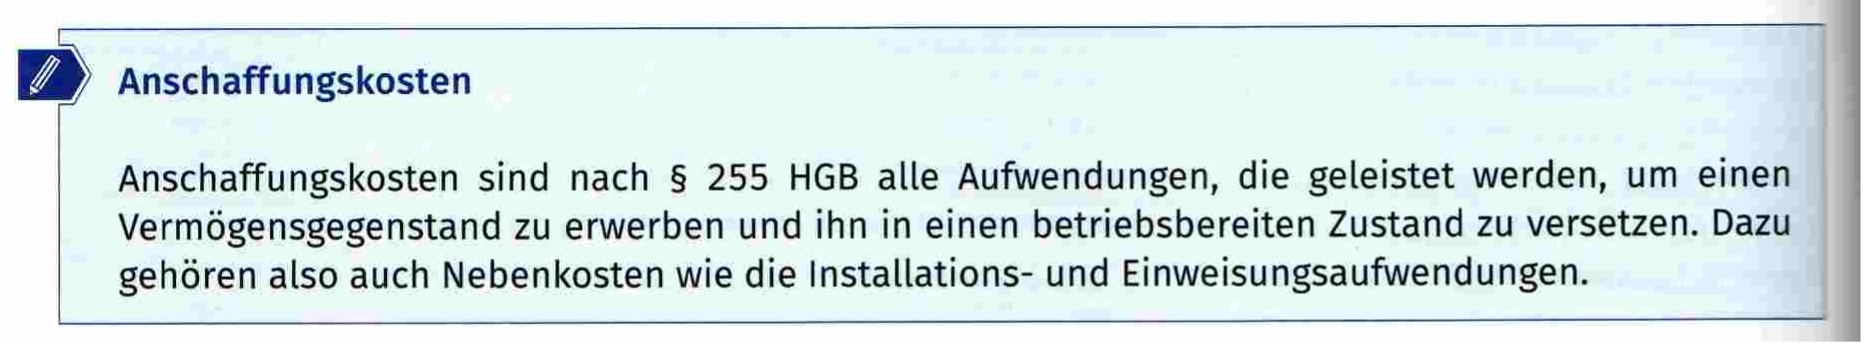
\includegraphics[width=12cm]{Anschaffungskosten.png}
    \end{center}
    \label{fig:Anschaffungskosten.png}
\end{figure}

Mit der Berechnung des TCO geht man noch weiter und bezieht alle Kosten ein.
Da dies Zahlen der Zukunft sind, werden sie in einer Kalkulationsentscheidung geschätzt. Dabei muss man indirekte und direkte Kosten unterscheiden.

TCO = Total Cost of Ownership
Total Costs: Energie, Reparatur, Wartungskosten, Organisationskosten, Schulungskosten, Verwaltungsaufwand, Entschädigung für entgangene Geschäfte usw.

ROI = Return on Investment
Es geht hier um die Rendite einer Investition. Voraussetzung für die Berechnung des ROIs ist, dass sich Rückflüsse ergeben und ermitteln lassen (innerhalb der Nutzungsdauer).

\subsection{Besitz und Eigentum}
Besitz: Besitz ist die tatsächliche Herrschaft / Verfügbarkeit über eine Sache oder ein Recht. Der Besitzer kann mit der Sache nur im Rahmen von Vereinbarungen mit dem Eigentümer verfahren. (z.B. Mieter)

Eigentum: Eigentum ist die rechtliche Herrschaft / Verfügbarkeit über eine Sache oder ein Recht. Der Eigentümer kann mit der Sache beliebig verfahren, sofern dadurch nicht die Rechte Dritter verletzt werden. (z.B. Vermieter)

\subsubsection{Möglichkeiten der Eigentumsübertragung}
\textbf{Bei beweglichen Sachen:}

Einigung und Übergabe:
Einigung zwischen Käufer und Verkäufer über die Übertragung des Eigentums im Rahmen des Erfüllungsgeschäftes und Übergabe, wenn der Gegenstand beim Verkäufer ist.\\
Beispiel: Der Verkäufer übergibt den gekauften Fotoapparat an den Käufer. Beide sind sich einig, dass das Eigentum übertragen wird.


Einigung: Käufer ist bereits Besitzer und wird durch die Einigung Eigentümer.
\begin{itemize}
    \item Beispiel: Nach Abschluss des Kaufvertrages wird der Käufer Eigentümer der vorher gemieteten Videoanlage (die sich in seinem Besitz befindet) nur aufgrund der Einigung über die Eigentumsübertragung. Eine Übergabe ist nicht mehr erforderlich.
\end{itemize}


Besitzkonstitut:
Einigung über die Eigentumsübertragung und Vereinbarung, dass der Verkäufer Besitzer bleibt.
\begin{itemize}
    \item Beispiel: Der Käufer erwirbt mehrere Wertpapiere von seiner Hausbank und belässt die Papiere weiterhin im Depot der Bank. Er wird Eigentümer der Wertpapiere durch die Vereinbarung, dass der Verkäufer weiterhin Besitzer bleibt und er das Eigentum erwirbt. (Käufer = mittelbarer Besitzer,- Verkäufer = unmittelbarer Besitzer)
\end{itemize}


Abtretung des Herausgabeanspruchs:
Einigung über die Eigentumsübertragung und Abtretung des Anspruchs auf Herausgabe der Sache, wenn sich der Gegenstand bei einem Dritten befindet.
\begin{itemize}
    \item Beispiel: Der Verkäufer überträgt das Eigentum an einem Familienzelt durch die Vereinbarung, dass der Käufer gegenüber seinem Freund, dem er zur Zeit das Zelt geliehen hat, einen Herausgabeanspruch hat
\end{itemize}

\textbf{Bei unbeweglichen Sachen:}

Auflassung (Einigung) und Eintragung in das Grundbuch:
Die Eintragung erfolgt, wenn die Auflassung nachgewiesen, die Eintragung beantragt und bewilligt wurde und die Bestätigung über die Zahlung der Grunderwerbssteuer vorliegt.

\textbf{Bei Rechten:}
Einigung über die Übertragung des Eigentums und Abtretung (=Zession)
Beispiel: Der Händler tritt seine Forderung an einen Kunden an seinen Lieferanten ab.

\textbf{Sonstiges:}

\textbf{Ersitzung:}
Ist eine bewegliche Sache zehn Jahre im Eigenbesitz, so erfolgt die Eigentumsübertragung.

\textbf{Fund:}
Der Finder erwirbt unter bestimmten Umständen mit dem Ablauf von sechs Monaten nach Anzeige des Fundes das Eigentum.

\textbf{Verarbeitung, Vermischung, Verbindung:}
Es ist möglich, das Alleineigentum an der Sache zu erwerben.

\textbf{Gutgläubiger Erwerb:}
Gutgläubiger Erwerb liegt vor, wenn der Veräußerer für den Eigentümer gehalten werden durfte. Der gutgläubige Eigentumserwerb ist jedoch nicht möglich bei gestohlenen, verloren gegangenen oder
sonst abhanden gekommenen Sachen (Ausnahme: Geld, Inhaberpapiere).

\subsection{AGB}
\begin{figure}[H]
    \begin{center}
        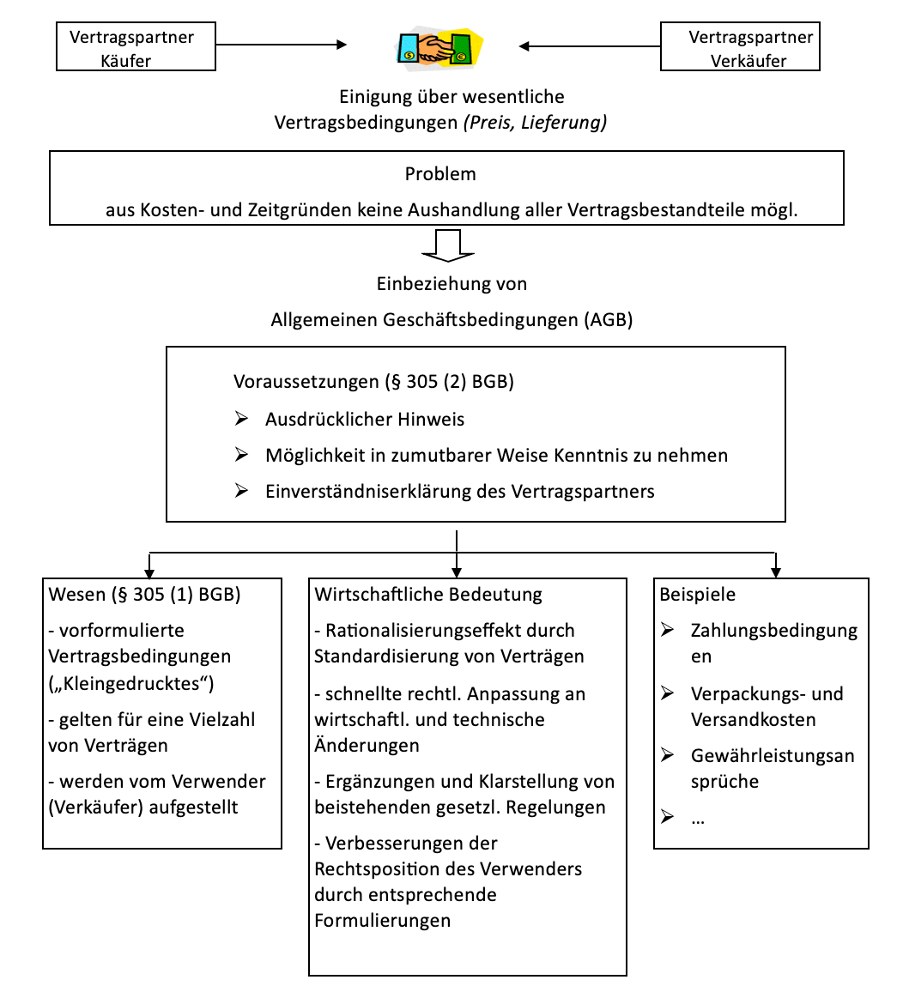
\includegraphics[width=12cm]{AGB.png}
    \end{center}
    \label{fig:AGB.png}
\end{figure}

Unzulässige Bestimmungen in Allgemeinen Geschäftsbedingungen (AGB)
\begin{itemize}
    \item[-] Unangemessene Benachteiligung des Käufers
    \item[-]  Überraschende (ungewöhnliche) Klauseln
    \item[-]  Preiserhöhungen innerhalb von 4 Monaten nach Vertragsabschluss
    \item[-] Eine Bestimmung über unbestimmte Liefertermine ist unwirksam
    \item[-]  Aufhebung oder Verkürzung der Gewährleistung für mangelfreie Ware
    \item[-]  Einschränkung von Gewährleistungsansprüchen
    \item[-] Verpflichtung des Käufers zu einer Vertragsstrafe
    \item[-]  Rücktritts- und Änderungsrecht des Verkäufers
    \item[-]   Ausschluss des Rechts des Käufers auf Rücktritt vom Vertrag bei mangelhafter Lieferung
\end{itemize}

\subsection{Fernabsatzverträge}
\begin{figure}[H]
    \begin{center}
        \includegraphics[width=12cm]{Fernabsatzverträge.png}
    \end{center}
    \label{fig:Fernabsatzverträge.png}
\end{figure}

\end{document}